% Lines starting with a percent sign (%) are comments. LaTeX will 
% not process those lines. Similarly, everything after a percent 
% sign in a line is considered a comment. To produce a percent sign
% in the output, write \% (backslash followed by the percent sign). 
% ==================================================================
% Usage instructions:
% ------------------------------------------------------------------
% The file is heavily commented so that you know what the various
% commands do. Feel free to remove any comments you don't need from
% your own copy. When redistributing the example thesis file, please
% retain all the comments for the benefit of other thesis writers! 
% ==================================================================
% Compilation instructions: 
% ------------------------------------------------------------------
% Use pdflatex to compile! Input images are expected as PDF files.
% Example compilation:
% ------------------------------------------------------------------
% > pdflatex thesis-example.tex
% > bibtex thesis-example
% > pdflatex thesis-example.tex
% > pdflatex thesis-example.tex
% ------------------------------------------------------------------
% You need to run pdflatex multiple times so that all the cross-references
% are fixed. pdflatex will tell you if you need to re-run it (a warning
% will be issued)  
% ------------------------------------------------------------------
% Compilation has been tested to work in ukk.cs.hut.fi and kosh.hut.fi
% - if you have problems of missing .sty -files, then the local LaTeX
% environment does not have all the required packages installed.
% For example, when compiling in vipunen.hut.fi, you get an error that
% tikz.sty is missing - in this case you must either compile somewhere
% else, or you cannot use TikZ graphics in your thesis and must therefore
% remove or comment out the tikz package and all the tikz definitions. 
% ------------------------------------------------------------------

% General information
% ==================================================================
% Package documentation:
% 
% The comments often refer to package documentation. (Almost) all LaTeX
% packages have documentation accompanying them, so you can read the
% package documentation for further information. When a package 'xxx' is
% installed to your local LaTeX environment (the document compiles
% when you have \usepackage{xxx} and LaTeX does not complain), you can 
% find the documentation somewhere in the local LaTeX texmf directory
% hierarchy. In ukk.cs.hut.fi, this is /usr/texlive/2008/texmf-dist,
% and the documentation for the titlesec package (for example) can be 
% found at /usr/texlive/2008/texmf-dist/doc/latex/titlesec/titlesec.pdf.
% Most often the documentation is located as a PDF file in 
% /usr/texlive/2008/texmf-dist/doc/latex/xxx, where xxx is the package name; 
% however, documentation for TikZ is in
% /usr/texlive/2008/texmf-dist/doc/latex/generic/pgf/pgfmanual.pdf
% (this is because TikZ is a front-end for PGF, which is meant to be a 
% generic portable graphics format for LaTeX).
% You can try to look for the package manual using the ``find'' shell
% command in Linux machines; the find databases are up-to-date at least
% in ukk.cs.hut.fi. Just type ``find xxx'', where xxx is the package
% name, and you should find a documentation file.
% Note that in some packages, the documentation is in the DVI file
% format. In this case, you can copy the DVI file to your home directory,
% and convert it to PDF with the dvipdfm command (or you can read the
% DVI file directly with a DVI viewer).
% 
% If you can't find the documentation for a package, just try Googling
% for ``latex packagename''; most often you can get a direct link to the
% package manual in PDF format.
% ------------------------------------------------------------------


% Document class for the thesis is report       
% ------------------------------------------------------------------
% You can change this but do so at your own risk - it may break other things.
% Note that the option pdftext is used for pdflatex; there is no
% pdflatex option. 
% ------------------------------------------------------------------
\documentclass[12pt,a4paper,oneside,pdftex]{report}

% The input files (tex files) are encoded with the latin-1 encoding 
% (ISO-8859-1 works). Change the latin1-option if you use UTF8 
% (at some point LaTeX did not work with UTF8, but I'm not sure
% what the current situation is) 
\usepackage[utf8]{inputenc}
% OT1 font encoding seems to work better than T1. Check the rendered
% PDF file to see if the fonts are encoded properly as vectors (instead
% of rendered bitmaps). You can do this by zooming very close to any letter 
% - if the letter is shown pixelated, you should change this setting 
% (try commenting out the entire line, for example).    
\usepackage[OT1]{fontenc}
% The babel package provides hyphenating instructions for LaTeX. Give
% the languages you wish to use in your thesis as options to the babel
% package (as shown below). You can remove any language you are not
% going to use.
% Examples of valid language codes: english (or USenglish), british, 
% finnish, swedish; and so on.
\usepackage[finnish,swedish,english]{babel}


% Font selection
% ------------------------------------------------------------------
% The default LaTeX font is a very good font for rendering your 
% thesis. It is a very professional font, which will always be 
% accepted. 
% If you, however, wish to spicen up your thesis, you can try out
% these font variants by uncommenting one of the following lines
% (or by finding another font package). The fonts shown here are 
% all fonts that you could use in your thesis (not too silly). 
% Changing the font causes the layouts to shift a bit; you many
% need to manually adjust some layouts. Check the warning messages
% LaTeX gives you.
% ------------------------------------------------------------------
% To find another font, check out the font catalogue from
% http://www.tug.dk/FontCatalogue/mathfonts.html
% This link points to the list of fonts that support maths, but
% that's a fairly important point for master's theses.
% ------------------------------------------------------------------
% <rant>
% Remember, there is no excuse to use Comic Sans, ever, in any
% situation! (Well, maybe in speech bubbles in comics, but there 
% are better options for those too)
% </rant>

% \usepackage{palatino}
% \usepackage{tgpagella}



% Optional packages
% ------------------------------------------------------------------
% Select those packages that you need for your thesis. You may delete
% or comment the rest.

% Natbib allows you to select the format of the bibliography references.
% The first example uses numbered citations: 
\usepackage[square,sort&compress,numbers]{natbib}
% The second example uses author-year citations.
% If you use author-year citations, change the bibliography style (below); 
% acm style does not work with author-year citations.
% Also, you should use \citet (cite in text) when you wish to refer
% to the author directly (\citet{blaablaa} said blaa blaa), and 
% \citep when you wish to refer similarly than with numbered citations
% (It has been said that blaa blaa~\citep{blaablaa}).
% \usepackage[square]{natbib}

% The alltt package provides an all-teletype environment that acts
% like verbatim but you can use LaTeX commands in it. Uncomment if 
% you want to use this environment. 
% \usepackage{alltt}

% The eurosym package provides a euro symbol. Use with \euro{}
\usepackage{eurosym} 

% Verbatim provides a standard teletype environment that renderes
% the text exactly as written in the tex file. Useful for code
% snippets (although you can also use the listings package to get
% automatic code formatting). 
\usepackage{verbatim}

% The listing package provides automatic code formatting utilities
% so that you can copy-paste code examples and have them rendered
% nicely. See the package documentation for details.
% \usepackage{listings}

% The fancuvrb package parovides fancier verbatim environments 
% (you can, for example, put borders around the verbatim text area
% and so on). See package for details.
% \usepackage{fancyvrb}

% Supertabular provides a tabular environment that can span multiple 
% pages. 
%\usepackage{supertabular}
% Longtable provides a tabular environment that can span multiple 
% pages. This is used in the example acronyms file. 
\usepackage{longtable}

% The fancyhdr package allows you to set your the page headers 
% manually, and allows you to add separator lines and so on. 
% Check the package documentation. 
% \usepackage{fancyhdr}

% Subfigure package allows you to use subfigures (i.e. many subfigures
% within one figure environment). These can have different labels and
% they are numbered automatically. Check the package documentation. 
\usepackage{subfigure}

% The titlesec package can be used to alter the look of the titles 
% of sections, chapters, and so on. This example uses the ``medium'' 
% package option which sets the titles to a medium size, making them
% a bit smaller than what is the default. You can fine-tune the 
% title fonts and sizes by using the package options. See the package
% documentation.
\usepackage[medium]{titlesec}

% The TikZ package allows you to create professional technical figures.
% The learning curve is quite steep, but it is definitely worth it if 
% you wish to have really good-looking technical figures. 
\usepackage{tikz}
% You also need to specify which TikZ libraries you use
\usetikzlibrary{positioning}
\usetikzlibrary{calc}
\usetikzlibrary{arrows}
\usetikzlibrary{decorations.pathmorphing,decorations.markings}
\usetikzlibrary{shapes}
\usetikzlibrary{patterns}


% The aalto-thesis package provides typesetting instructions for the
% standard master's thesis parts (abstracts, front page, and so on)
% Load this package second-to-last, just before the hyperref package.
% Options that you can use: 
%   mydraft - renders the thesis in draft mode. 
%             Do not use for the final version. 
%   doublenumbering - [optional] number the first pages of the thesis
%                     with roman numerals (i, ii, iii, ...); and start
%                     arabic numbering (1, 2, 3, ...) only on the 
%                     first page of the first chapter
%   twoinstructors  - changes the title of instructors to plural form
%   twosupervisors  - changes the title of supervisors to plural form
\usepackage[mydraft]{aalto-thesis}
%\usepackage[mydraft,doublenumbering]{aalto-thesis}
%\usepackage{aalto-thesis}


% Hyperref
% ------------------------------------------------------------------
% Hyperref creates links from URLs, for references, and creates a
% TOC in the PDF file.
% This package must be the last one you include, because it has
% compatibility issues with many other packages and it fixes
% those issues when it is loaded.   
\RequirePackage[pdftex]{hyperref}
% Setup hyperref so that links are clickable but do not look 
% different
\hypersetup{colorlinks=false,raiselinks=false,breaklinks=true}
\hypersetup{pdfborder={0 0 0}}
\hypersetup{bookmarksnumbered=true}
% The following line suggests the PDF reader that it should show the 
% first level of bookmarks opened in the hierarchical bookmark view. 
\hypersetup{bookmarksopen=true,bookmarksopenlevel=1}
% Hyperref can also set up the PDF metadata fields. These are
% set a bit later on, after the thesis setup.   


% Thesis setup
% ==================================================================
% Change these to fit your own thesis.
% \COMMAND always refers to the English version;
% \FCOMMAND refers to the Finnish version; and
% \SCOMMAND refers to the Swedish version.
% You may comment/remove those language variants that you do not use
% (but then you must not include the abstracts for that language)
% ------------------------------------------------------------------
% If you do not find the command for a text that is shown in the cover page or
% in the abstract texts, check the aalto-thesis.sty file and locate the text
% from there. 
% All the texts are configured in language-specific blocks (lots of commands
% that look like this: \renewcommand{\ATCITY}{Espoo}.
% You can just fix the texts there. Just remember to check all the language
% variants you use (they are all there in the same place). 
% ------------------------------------------------------------------
\newcommand{\TITLE}{Clustering of Finnish scientific publications 
by discipline}
\newcommand{\FTITLE}{Suomalaisten tieteellisten julkaisujen 
ryhmittely tieteenaloittain klusteroimalla}
\newcommand{\STITLE}{Klustring av finländska vetenskapliga 
publikationer efter disciplin}
\newcommand{\SUBTITLE}{No subtitle}
\newcommand{\FSUBTITLE}{Ei alaotsikkoa}
\newcommand{\SSUBTITLE}{Igen undertitel}
\newcommand{\DATE}{November 30, 2017}
\newcommand{\FDATE}{30. marraskuuta 2017}
\newcommand{\SDATE}{Den 30 November 2017}

% Supervisors and instructors
% ----------------------------------------------------------------
% If you have two supervisors, write both names here, separate 
% them with a double-backslash (see below for an example)
% Also remember to add the package option ``twosupervisors'' or
% ``twoinstructors'' to the aalto-thesis package so that the 
% titles are in plural.
% Example of one supervisor:
%\newcommand{\SUPERVISOR}{Professor Antti Yla-Jaaski}
%\newcommand{\FSUPERVISOR}{Professori Antti Yla-Jaaski}
%\newcommand{\SSUPERVISOR}{Professor Antti Yla-Jaaski}
% Example of twosupervisors:
\newcommand{\SUPERVISOR}{Professor Samuel Kaski}
\newcommand{\FSUPERVISOR}{Professori Samuel Kaski}
\newcommand{\SSUPERVISOR}{Professor Samuel Kaski}

% If you have only one instructor, just write one name here
\newcommand{\INSTRUCTOR}{Yrjö Leino Lic.Sc. (Tech.)}
\newcommand{\FINSTRUCTOR}{Tekniikan lisensiaatti Yrjö Leino}
\newcommand{\SINSTRUCTOR}{Teknologie licentiat Yrjö Leino}
% If you have two instructors, separate them with \\ to create 
% linefeeds
% \newcommand{\INSTRUCTOR}{Olli Ohjaaja M.Sc. (Tech.)\\
%  Elli Opas M.Sc. (Tech)}
% \newcommand{\FINSTRUCTOR}{Diplomi-insinoori Olli Ohjaaja\\
%  Diplomi-insinoori Elli Opas}
% \newcommand{\SINSTRUCTOR}{Diplomingenjor Olli Ohjaaja\\
%  Diplomingenjor Elli Opas}

% If you have two supervisors, it is common to write the schools
% of the supervisors in the cover page. If the following command 
% is defined, then the supervisor names shown here are printed in 
% the cover page. Otherwise, the supervisor names defined above 
% are used.
% \newcommand{\COVERSUPERVISOR}{Professor Antti Yla-Jaaski, Aalto 
%University\\
%  Professor Pekka Perustieteilija, University of Helsinki}

% The same option is for the instructors, if you have multiple 
% instructors.
% \newcommand{\COVERINSTRUCTOR}{Olli Ohjaaja M.Sc. (Tech.), Aalto 
% University\\ Elli Opas M.Sc. (Tech), Aalto SCI}


% Other stuff
% ----------------------------------------------------------------
\newcommand{\PROFESSORSHIP}{Computer Science}
\newcommand{\FPROFESSORSHIP}{Tietojenkäsittelytiede}
\newcommand{\SPROFESSORSHIP}{Datavetenskap}
% Professorship code is the same in all languages
\newcommand{\PROFCODE}{SCI3042}
\newcommand{\KEYWORDS}{clustering, bibliomterics}
\newcommand{\FKEYWORDS}{ryvästys, bibliometriikka}
\newcommand{\SKEYWORDS}{klusteranalys, bibliometri}
\newcommand{\LANGUAGE}{English}
\newcommand{\FLANGUAGE}{Englanti}
\newcommand{\SLANGUAGE}{Engelska}

% Author is the same for all languages
\newcommand{\AUTHOR}{Juho Lehtonen}


% Currently the English versions are used for the PDF file 
% metadata
% Set the PDF title
\hypersetup{pdftitle={\TITLE\ \SUBTITLE}}
% Set the PDF author
\hypersetup{pdfauthor={\AUTHOR}}
% Set the PDF keywords
\hypersetup{pdfkeywords={\KEYWORDS}}
% Set the PDF subject
\hypersetup{pdfsubject={Master's Thesis}}


% Layout settings
% ----------------------------------------------------------------

% When you write in English, you should use the standard LaTeX 
% paragraph formatting: paragraphs are indented, and there is no 
% space between paragraphs.
% When writing in Finnish, we often use no indentation in the
% beginning of the paragraph, and there is some space between the 
% paragraphs. 

% If you write your thesis Finnish, uncomment these lines; if 
% you write in English, leave these lines commented! 
% \setlength{\parindent}{0pt}
% \setlength{\parskip}{1ex}

% Use this to control how much space there is between each line of
% text. 1 is normal (no extra space), 1.3 is about one-half more 
% space, and 1.6 is about double line spacing.  
% \linespread{1} % This is the default
% \linespread{1.3}

% Bibliography style
% acm style gives you a basic reference style. It works only with 
% numbered references.
\bibliographystyle{acm}
% Plainnat is a plain style that works with both numbered and name
% citations.
% \bibliographystyle{plainnat}


% Extra hyphenation settings
% ----------------------------------------------------------------
% You can list here all the files that are not hyphenated 
% correctly. You can provide many \hyphenation commands and/or 
% separate each word with a space inside a single command. Put 
% hyphens in the places where a word can be hyphenated.
% Note that (by default) LaTeX will not hyphenate words that 
% already have a hyphen in them (for example, if you write 
% ``structure-modification operation'', the word 
% structure-modification will never be hyphenated). You need a 
% special package to hyphenate those words.
\hyphenation{di-gi-taa-li-sta yksi-suun-tai-sta}



% The preamble ends here, and the document begins. 
% Place all formatting commands and such before this line.
% ----------------------------------------------------------------
\begin{document}
% This command adds a PDF bookmark to the cover page. You may 
% leave it out if you don't like it...
\pdfbookmark[0]{Cover page}{bookmark.0.cover}
% This command is defined in aalto-thesis.sty. It controls the 
% page numbering based on whether the doublenumbering option is 
% specified
\startcoverpage

% Cover page
% ----------------------------------------------------------------
% Options: finnish, english, and swedish
% These control in which language the cover-page information is 
% shown
\coverpage{english}


% Abstracts
% ----------------------------------------------------------------
% Include an abstract in the language that the thesis is written 
% in, and if your native language is Finnish or Swedish, one in 
% that language.

% Abstract in English
% ----------------------------------------------------------------
\thesisabstract{english}{
\fixme{Abstract text here.} 
% Fixme is a command that helps you identify parts of your thesis 
% that still require some work. When compiled in the custom 
% \texttt{mydraft} mode, text parts tagged with fixmes are shown 
% in bold and with fixme tags around them. When compiled in 
% normal mode, the fixme-tagged text is shown normally (without
% special formatting). The draft mode also causes the ``Draft'' 
% text to appear on the front page, alongside with the document 
% compilation date. The custom \texttt{mydraft} mode is selected 
% by the \texttt{mydraft} option given for the package 
% \texttt{aalto-thesis}, near the top of the 
% \texttt{thesis-example.tex} file.
}

% Abstract in Finnish
% ----------------------------------------------------------------
% E: Package babel Error: You haven't defined... ??
% S: sudo dnf install -y texlive-babel-finnish
% E: Package babel Warning: No hyphenation patterns were 
%    preloaded for the language `Finnish' into the format.
% S: Ei viela nailla korjaantunut. Tasta voi jatkaa.
%    sudo dnf install -y texlive-hyphen-finnish
%    sudo texhash
%    sudo fmtutil-sys --refresh
%    sudo fmtutil -sys --all
%    sudo fmtutil -sys --listcfg
\thesisabstract{finnish}{
Suomekielinen tiivistelmä
}


% Abstract in Swedish
% ----------------------------------------------------------------
\thesisabstract{swedish}{
Svensk text här.
}


% Acknowledgements
% ----------------------------------------------------------------
% Select the language you use in your acknowledgements
\selectlanguage{english}

% Uncomment this line if you wish acknoledgements to appear in the 
% table of contents
%\addcontentsline{toc}{chapter}{Acknowledgements}

% The star means that the chapter isn't numbered and does not 
% show up in the TOC
\chapter*{Acknowledgements}

Some acknowledgements here...

Thank you...
\vskip 10mm

\noindent Espoo, \DATE
\vskip 5mm
\noindent\AUTHOR

% Acronyms
% ----------------------------------------------------------------
% Use \cleardoublepage so that IF two-sided printing is used 
% (which is not often for masters theses), then the pages will still
% start correctly on the right-hand side.
\cleardoublepage
% Example acronyms are placed in a separate file, acronyms.tex
\addcontentsline{toc}{chapter}{Abbreviations and Acronyms}
\chapter*{Abbreviations and Acronyms}

% The longtable environment should break the table properly to multiple pages, 
% if needed

\noindent
\begin{longtable}{@{}p{0.25\textwidth}p{0.7\textwidth}@{}}
LSA & Latent semantic analysis \\
MDS & Multi-dimensional scaling \\
SVD & Singular value decomposition \\
tf-idf & term frequency-inverse document frequency \\
note & Note also, that this list is not compulsory, and should be 
omitted if you have only few abbreviations \\

\end{longtable}


% Table of contents
% ----------------------------------------------------------------
\cleardoublepage
% This command adds a PDF bookmark that links to the contents.
% You can use \addcontentsline{} as well, but that also adds contents
% entry to the table of contents, which is kind of redundant.
% The text ``Contents'' is shown in the PDF bookmark. 
\pdfbookmark[0]{Contents}{bookmark.0.contents}
\tableofcontents

% List of tables
% ------------------------------------------------------------------
% You only need a list of tables for your thesis if you have very 
% many tables. If you do, uncomment the following two lines.
% \cleardoublepage
% \listoftables

% Table of figures
% ------------------------------------------------------------------
% You only need a list of figures for your thesis if you have very 
% many figures. If you do, uncomment the following two lines.
% \cleardoublepage
% \listoffigures

% The following label is used for counting the prelude pages
\label{pages-prelude}
\cleardoublepage

%%%%%%%%%%%%%%%%% The main content starts here %%%%%%%%%%%%%%%%%%%%%
% ------------------------------------------------------------------
% This command is defined in aalto-thesis.sty. It controls the page 
% numbering based on whether the doublenumbering option is specified
\startfirstchapter

% Add headings to pages (the chapter title is shown)
\pagestyle{headings}

% The contents of the thesis are separated to their own files.
% Edit the content in these files, rename them as necessary.
% ------------------------------------------------------------------
\chapter{Introduction}
\label{chapter:intro}
% The target
% ==========
This thesis handles the problem of clustering Finnish scientific 
publications by their metadata. The target is to cluster 
them as well as possible by their scientific discipline. \fixme{
Tahan enemman tavoitteen kuvausta ei viela maarittelyn vaikeutta.}
Of course 
the ``wellness'' of a clustering measured by how it fits to 
scientific fields is a tricky issue for at least couple of 
reasons.


% Obstacles
% =========
First, there is no general consensus about what is the correct 
partition of all science to different branches. It might be depend 
on specific need or individual opinion where the line between two 
related discipline lies.

Second, science is evolving all the time. What was yesterday seen 
simply as chemistry could today be viewed as organic and inorganic 
chemistry.

Third, the definition of scientific disciplines depends also how 
closely we look into a topic. Sometimes chemistry is sufficent 
description for eg. a publication and sometimes we need to define 
it more accurately as organic chemistry.
% LMa: Tahan maininta poikkitieteellisten alojen 
% ongelmallisuudesta, onko bioinformatiikka, biologiaa, 
% tietotekniikkaa vai oma tieteenalansa.

But despite this ambiguousness of the target we define and 
justify some goals and how to measure our success.


% Environment/background
% ======================
In Finland there are 15 universities and 23(+2) universities of 
applied sciences. Additionally there are 12 research institutes.
Each year Finnish scientific efforts produce about 
10000 publications in all scientific disciplines. 
\fixme{10000 tulee siis WOS ja Elsevierilta} The Ministry of 
Education and Culture oversees what is researched and in what 
quanities in the Finnish research.
Classifying articles by discipline enables different types of 
bibliometric analysis.
% It is also ill posed problem because there is no one right answer
% for the problem. Different tasks require different classification.
Because of the amount of the scientific articles manual 
classification is not applicable. \fixme{Also: kukaan tuskin 
pystyy hallitsemaan kaikkia tieteenaloja. Tavoitteena tyokalu, 
jolla analyysin tekija voi luokitella }
% All these are manual methods. Automatic methods are needed...
Automatic methods should be able to label the article by some 
criterion to the (subjectively) obvious discipline. The input for 
automatic method can usually at most be the whole article and 
perhaps some metadata describing it. The metadata can be 
created by the author or the publisher or some archive.

\fixme{What methods used?}
Different methods have been suggested. NN1 suggested SOME METHOD. 
NN2 suggested SOME OTHER METHOD. NN3 suggested YET A METHOD.

In this thesis we will try to cluster Finnish publications by 
discipline by using the metadata.





\section{Problem statement}

Refactor from above...

\section{Structure of the Thesis}
\label{section:structure} 

% Use transition in your text, meaning that you should help
% the reader follow the thesis outline. Here, you tell what will be in
% each chapter of your thesis.
In chapter 2. we will shortly present the background...


\chapter{Background}
\label{chapter:background}

% Tiedonhankintaa suunnitellessasi voi miettiä vastauksia mm. 
% seuraaviin aiheen määrittelyä selventäviin tutkimuskysymyksiin:
% 
%     Mistä aiheesta tietoa tarvitaan?
%       bibliometriikasta, sen määritelmästä sekä klusteroinnista
%     Mihin tarkoitukseen tietoa tarvitaan?
%       Aiheen taustan kuvailuun, menetelmien kuvailuun ja 
%       valitun menetelmän toteuttamiseen
%     Mikä aiheessa on keskeistä?
%       Klusterointimenetelmän kokeilu ja tulosten raportointi
%     Mistä näkökulmasta aihetta lähestytään?
%       Käytännön implementaation kokeilulla
%     Mitä aiheesta tiedetään jo ennalta?
%       Klusteroinnista perusteet, bibliometriikasta vähemmän
%     Tarvitaanko yleis- vai tieteellistä tietoa?
%       Bibliometriikasta tarvitaan vähän yleistietoa, 
%       klusteroinnista tieteellistä.
%     Tarvitaanko kuva-aineistoa?
%       Ei muuta kuin itse tuotetut
%     Minkä ikäistä tietoa tarvitaan?
%       Yleis- ja taustatiedot vanhoista asioista, aiheen 
%       oleellinen tieto uusinta
%     Minkä kielistä tietoa tarvitaan?
%       suomi ja englanti käy


In this chapter we briefly introduce clustering and how it is 
positioned in the larger field of machine learning. But first we
describe what bibliometrics is.
% Taman esittelyjarjestyksen voi vaihtaa myohemmin

\section{Bibliometrics}
\label{sec:bibliometrics}
% Mita bibliometriikka on?
% Valmis --->-v
Bibliometrics is a study of written scientific records. The 
records may be books, articles, letters in scientific journals, 
conference papers and so on. Bibliometrics studies how these 
products of research are communicated, how are they related to 
each other, what kind of properties they have and what can be 
learned about the science in general by analysing them.

% Mihin bibliometriikka pyrkii vastaamaan?
Bibliometrics seeks to answer questions like ``How many 
publications has an author authored?'', ``How many citations an 
author has'', ``What are the 
cited publications of a scientific document?''. It also studies
a bit more boarder questions like ``How many publications
on discipline X been published a year?'', ``Which research area
does this publication belong to?'', ``What other publications 
belong to this research area?'', ``When has this research area
emerged?'', ``What are the most important related research areas
of this discipline?'' an so on.

% Background/history
% ==================
% Mika bibliometriikan historia on?
% OK --->-v
Classifying things is often the first thing we do when we observe 
the world. On the other hand, counting the frequenzies of objects
and comparing these numbers often helps to put things in 
perspective.
% Tahan voisi laittaa sidontaa todennakoisyyslaskennalla tjsp.
One of the earliest studies that is generally considered
bibliometrics was Cole's and Eales' analysis to the anatomy 
literature in 1917 \cite{cole_history_1917}. In this study they 
researched the anatomy literature from 1543 through 1860 with the 
intention to graph the growth of of the number of documents over 
the three centuries, to present ``the performance'' of each 
European country, to observe the most popular topics among 
scholars from time to time, and to compare the advancement and 
devolution stages of the research with different societal 
events \cite{bellis_bibliometrics_2009}.
As the number of scientific publications has enormously increased
the need to automatically analyze them has become apparent.
The basic analysis on top of which more detailed studies can be 
built on is classifying each publication to research areas and
disciplines.
% The need for some kind of bibliometric indices rise in the 
% First modern(?) classification was... by... some 
% indexing/publishing/to facilitate communication...
% At some point more and more automation was needed for bibliomterics
% There has been lot of study in automatically classificating the 
% science. 


\subsection{Classification in bibliometrics}
% Specific charasteristics of classifying the bibliometrics
% Miten bibliometriikkaa voidaan jasentaa / mista se koostuu?
% Existing classification systems / methods
% =========================================
\fixme{Onko Scopus tässä relevantti jos ei Scopus-dataa?}
Currently, the most popular systems to classify the publications 
into research areas are the Clarivate's (formerly Thomson Reuters)
Web of Science and Elsevier's Scopus classification
systems. These classification systems classify the journals into
one or more research areas. \cite{waltman_new_2012} Publications
are then classified to research areas based on in which journal they
were published. WoS uses approximately 250 \emph{subject categories}
in its classification. Each journal can belong 
to one or up to six categories. The categories have been created
at least or before early 1960's by manually classifying journals.
New journals were added one at the time after visual inspection of
citation information. New categories were added when when old ones
grew \cite{pudovkin_algorithmic_2002}. As for Scopus, according to 
Wang and Waltman \cite{wang_large-scale_2016}, ``there seems to be no 
information at all on the construction of its classification 
system''.

Also an independent journal level classification system has been 
developed. \cite{archambault_towards_2011}
Journal level classification systems have known limitations.
They are, for example, unable to meaningfully classify
publications published in multidiscipline journals.
Also some discipline specific classification systems exists such 
as (check them...).
An alternative classification system is publication level 
classification where each publication is classified based on some 
information extracted directly from the publication self such as
words used in the title and/or abstract, keywords attached by the
authors or publisher or citations to other publications.
Shu et al. have compared journal and paper level classification
approaches and found that publication level classification could
provide better classification \cite{shu_comparing_2019}.
% Usually classification of publications or journals can be approached 
% at least from multiple directions. There is clustering based method,
% the network based method and the combination of the two.
% In the network method

% ACM:n luokittelujärjestelmä esimerkkinä? CLSF?...
Bibliometric research 
uses mainly three types of methods; citation based, text analysis 
based or combination of the two \cite{janssens_hybrid_2009}.
Citation based methods study citations of publications and produce
networks where publications are nodes connected by citations as 
edges. In
 the rare case of publication having a direct quote including a
 citation, the citation is not counted unless it is also a
 citation of the publication itself.
Connection between two publications can be 
formed by a direct citation, bibliometric coupling where 
publications are connected when a third publication cites them 
both or co-citations where publications are connected if they 
cite the same third publication.

Text analysis based methods examine the title, the abstract or 
the whole text content of the publication itself and classify 
the publications or journals by the topic model created 
\cite{blei_latent_2003}.
Hybrid models combine both approaches. Authors and their
affilations are not used in this work because we cannot uniquely
identify them and we can't assume their field of science that is
our interest here.

% Tama on kompelosti ilmaistu, korjaa
% Verkkoanalyysin nakokulma
% These research products and relations between them form a 
% network that can reveal something about the structure of 
% different scientific disciplines. Finding the structure of this 
% kind of data set is called classification or clustering.


% Previous results using clustering bibliometrics
% ===============================================
% Kirjoitettu yllä olevaan


\subsection{Bibliometrics in Finland}
Ministry of Education and Culture of Finland provides yearly
updated bibliometric analyses of Finnish research activities 
based on both Web Of Science citation index 
and Elsevier's Scopus database \cite[Vipunen 
service]{noauthor_ministry_2019}. The corresponding source 
system classification for a field of science is used and
aggregated to match the Statistics Finland classification 
\cite{auranen_tieteen_2018}. CSC - 
IT Center for Science is responsible of the actual technical 
implementation of the service.

One of the earlier and comprehensive bibliometric research of 
Finnish science is a report by Persson et al. 
\cite{persson_bibliometric_2000} which mapped the situation and 
development of Finnish science 1981-1998.
This, however, is a report which concentrates on bibliometric 
analysis based on the map of science provided by WoS subject 
categories. But if we want to explore how the Finnish scientific 
disciplines themselves have evolved over time these pre-defined 
subject categories are quite rigid framework. For that reason we 
want to experiment creating an alternative mapping of science by 
clustering. 

So, as opposed to bibliometric analyses seeking to understand the
state of a scientific discipline as defined by some existing 
definition, we want to experiment/inspect how to define 
scientific disciplines to be used in bibliometric analyses.

%Efforts to cluster Finnish research include a study by...

Suominen and Toivanen used unsupervised learning-based topic 
modeling to create a map of science for Finnish publications from 
1995-2011. They evaluated it by comparing the results with WoS 
based classification and concluded that superiority of the method
depends on the purpose of analysis. Traditional manually created 
classifications are relevant for information retrieval while 
machine learning methods can reveal new emerging areas of science 
\cite{suominen_map_2016}. Compared to our work here, their 
analysis method topic modeling differs from hierarchical 
clustering albeit both are unsupervised learning methods.
\fixme{Vie myös ``Discussion'' -osioon.}

Our research question here is: "How to automatically cluster 
Finnish scientific publications and how does that clustering 
compare to existing fiels of science classification by WoS?" We 
will use hierarchical clustering on features derived from titles,
abstracts and keywords in publication metadata.


\section{Clustering}
The methods discussed in this work belong to the field of machine 
learnig. The field has it's roots in statistics and engineering 
and is itself part of artificial intelligence.
The methods in machine learnig can be divided to supervised, 
unsupervised and reinforced learning \cite{alpaydin2004introduction}.

Commonly for all methods we define $X$ as
the sample data and $Y$ as label indicating which class our data 
sample $X$ belongs. We also have to choose the model $f()$ for
learning from the data. Then we can state our learning problem as
a function $Y = f(w \cdot X)$, where $w$ is a weight vector, 
which would give a prediction of the class $Y$ of the sample data
$X$. 
Assuming we have enough of samples $X$ we then teach our model 
with training data. That is, we solve the weights $w$ using the
loss function such that it optimizes the difference between the 
true and predicted class labesl $Y$.

Supervised learnig methods include classification and continuous 
estimation (regression)
where the class of the training samples, or the target values in 
case of regression, $Y$ is known. Example of a classification 
problem is optical character recognition where the system is 
taught with example of characters along with their correct labels.

For unsupervised learning the correct answer or the label $Y$ is not known. 
Instead a model is applied such that it finds regularities in the
input data $X$. Example of unsupervised learning problem is 
finding anomalities that don't fit in the group, such as analysing
log files of a computer system to find a possible intruder.

Unsupervised learning methods include clustering, dimensionality
reduction and topic modeling for instance. Clustering try to 
distinguish patterns in the data and discriminate unrelated 
objects into separate clusters and aggregate related objects into
same cluster.

In reinforced learning we want the system to learn a sequence of
actions leading to desired outcome. For example we may want the 
system to learn to win a game. In that case individual actions
are not important but the end result as there are many ways to win
a game. So the system repaeatedly tries different combinations of
actions while it receives the result of it's combined actions.

\subsubsection{Model selection}
Generally all machine learning problems are ill-posed in the sense 
that a unique solution for the problem can't be found unless some
assumptions, or \emph(inductive bias), are introduced. This begins 
with selecting the learning algorithm.

Here we will unsupervised learning to shape a mapping of 
scientific disciplines because we want to learn the possible 
intristic structure of sciencetific knowledge. We will use 
clustering because it's quite simple and familiar to us. 
There are many different clustering algorithms from which to 
choose. Some often used common algorithms are k-means, hierarchical
clustering, density based scan clustering and Gaussian clustering.
We will use hierarchical clustering. Among the hierarchical 
clustering there are yet different parameters to choose. 
clustering as our method because clustering methods with different linkages applied 
to search query results are experimented by Korenius et al. 
\cite{korenius_hierarchical_2006}.

\fixme{Ero verkkoanalyysiin: lyhyesti}


\subsection{Choosing the number of clusters}
\fixme{Yleisellä tasolla: "tämän tyyppisiä menetelmiä on 
olemassa", "ne soveltuvat tähän ja tähän käyttötarkoitukseen". 
Helppo löytää ja käyttää viitteitä; esim. käytetty siinä ja siinä, 
meta- ja review-tutkimukset}
% 29.4.2020 Lyhyesti vain

In hierarchical clustering number of clusters can be chosen after 
the data has been clustered and the dendogram \fixme{explain more}
 formed.
\fixme{citation} By 
looking the dendrogram and using different metrics the number of 
clusters can be chosen.


\subsection{Evaluating of clustering results}
We will use Calinski \& Harabazt criterion (or the variance ratio 
criterion (VRC)) as an evaluation criterion for 
deciding the number clusters \cite{calinski_dendrite_1974}. It 
is defined as
\begin{equation}
 VRC_k = \frac{SS_B}{N-k} \frac{SS_W}{k-1},
\end{equation}
where $SS_B$ is the overall variance between clusters, $SS_W$ is 
the over variance within clusters, $k$ is the number of clusters 
and $N$ is the number of observations.

The overall variance between clusters $SS_B$ is defined as
\begin{equation}
 SS_B = \sum_{i=1}^k n_i ||m_i-m||^2,
\end{equation}
where $k$ is the number of clusters, $n_i$ is the number of 
observations in cluster $i$, $m_i$ is centroid of cluster $i$, 
$m$ is the overall mean of the sample data and $||m_i-m||$ is the 
Euclidean distance between the two vectors.

The overall variance within clusters $SS_W$ is defined as
\begin{equation}
 SS_W = \sum_{i=1}^k \sum_{x\in c_i} ||x-m_i||^2,
\end{equation}
where $k$ is the number of clusters, $x$ is the oservation, 
$c_i$ is the $i$th cluster, $m_i$ is centroid of cluster $i$, and 
$||x-m_i||$ is the Euclidean distance between the two vectors.
The larger the Calinski \& Harabazt criterion, the better the 
cluster structure.
\fixme{Tämä suoraan: 
https://www.mathworks.com/help/stats/clustering.evaluation.calinsk
iharabaszevaluation-class.html pitäisikö kertoa ``omin sanoin''?}



\subsubsection{Manually annotated validation set}
% Gold standard set. Actually a gold standard set would be a set
% of all data sets with abstract excluding sets that don't have it.
We will create a manually annotated validation set for calculating
precision, recall and metrics derived from those.
% määrittele peruskäsitteet kuten precision ja recall
The validation
set consists of $500$ publications from three different fields of
science, two more similar sub fields of computer science, 
information systems and artificial intelligence, and one more
distant from those, clinical neurology.

Publications are inspected by title, abstract, keywords, journal
and publisher assigned disciplines of the journal. We checked 
just by layman's reasoning if the labeled discipline seemed 
plausible. Because of the journal based 
classification, most publications had more than one 
assigned discipline. Only discipline labels named 
previously were retained because we were wanted test 
how well our clustering method separated these three 
groups regardless their labels. So essentially the 
labels could have been eg. 1, 2, 3. Publications
with critically missing data, unclear discipline assignment and
heavily applied publications were excluded from validation set.
Goal was to achieve evaluation measurements based on a quite 
clearly separated set of publications. More vaguely classifiable
publications were included for comparison. We asked an another 
opinion for publications that could have been in more 
than one of our categories. For manually curated validation set 
with discipline assignment and justifications for
possible exclusion see appendix (Insert reference!).

The basic problem is that fields of science can not be 
defined so that they clearly differ from each other. Where one 
discipline end the other has already started like metallurgy and 
material science. Likewise, there are lots of publications that 
handle topics belonging to more than one discipline, eg. this 
thesis discusses clustering and bibliometrics. So when annotating 
publications, deciding if a publication belonged to
a discipline or not felt often quite difficult. Often the 
separation between disciplines felt quite arbitrary. For example
an article describing using wavelet transformation for coding noisy
images was decided to belong to CS information systems whereas an
article describing wavelet based corner detection using SVD was
decided to belong to CS artificial intelligence.
For CS artificial intelligence we mostly selected publications 
which
mentioned some dimensionalty reduction or machine learning related
term or concept.
CS information systems ended up being quite like some ``others'' 
or
``the rest'' dump class. It would have publications such as
``A reference model for conceptualising the convergence of 
telecommunications and datacommunications service platforms'',
``Developing a distributed meeting service to support mobile 
meeting participants'',
``On voice quality of IP voice over GPRS'',
\fixme{Perustele vain yhteen alaan luokittelu. ``Tukeudun 
WOS-luokitteluun''.}
\fixme{Selvennä yläluokka-alaluokka-jako: CS general vs. CS 
information system tai CS artificial intelligence.}


%\chapter{Bibliometric}
\label{chapter:environment}

A problem instance is rarely totally independent of its environment.
Most often you need to describe the environment you work in, what
limits there are and so on. This is a good place to do that. First we
tell you about the LaTeX working environments and then is an example
from an thesis written some years ago.


\section{Clustering}
\label{sec:environments}



\subsection{Environment}







\chapter{Data and Methods}
\label{chapter:methods}
In this chapter we present the data and methods used in the 
clustering. We follow the logical order in which the methods are 
applied on the data. We first describe the raw data and  
pre-processing it. Then we explain the feature extraction 
transforming irregular length symbolic data (text) into numerical 
vector representation. Next to follow is reducing the 
dimensionality of the data, selecting the model used to learn from 
the data and finally the selected clustering method.

\section{Publication meta data}
\label{section:metadata}
The data consists of $21155$ records of Clarivate's Web of Science 
publication meta data from years 2000-2001. Each record describes some 
basic information about an article published in a scientific 
journal. The data contains only publications with at least one
author with an affiliation to a Finnish research organisation as
recorded in the publication. These publications were published in 
total in $2539$ different scientific journals.
An example of a shortened record:
\begin{verbatim}
 Lehti: ACTA OPHTHALMOLOGICA SCANDINAVICA
 ISSN: 1395-3907
 Ala: OPHTHALMOLOGY
 Ilmestymisvuosi:   1999
 Otsikko: Assessment of diabetic retinopathy using two-field 60 
 degrees fundus photography. A comparison between[...]
 Abstrakti
 Purpose: To assess the severity of diabetic retinopathy and 
 maculopathy bycomparing[...]
 Avainsana (KeywordPlus):  OPHTHALMOSCOPY
 Avainsana (KeywordPlus):  KAPPA
 [...]
 Avainsana (tekijät):  diabetic retinopathy
 Avainsana (tekijät):  diabetic maculopathy
 [...]
 Lähde: 0010603696 /  *DIAB CONTR COMPL /  NEW ENGL J MED /  977 
 /  329 /  1993
 Lähde: 0034118371 /  *DIAB CONTR COMPL /  ARCH OPHTHALMOL-CHI /  
 1344 /  105 /  1987
 Lähde: 0075276068 /  *DRS RES GROUP /  OPHTHALMOLOGY /  82 /  85 
 /  1978
 \end{verbatim}
 
Each meta data record contains a single instance of the title 
(``\texttt{Lehti}''), ISSN (International Standard Serial Number), 
the field of science (``\texttt{Ala}'') and publication year 
(``\texttt{Ilmestymisvuosi}'') of the journal, the title 
(``\texttt{Otsikko}'') and the abstract (``\texttt{Abstrakti}'') 
of the article. Additionally each meta data record can contain
multiple instances of keywords inferred by the publisher programmatically
(``\texttt{Avainsana (KeywordPlus)}''), keywords produced by the 
authors themselves (``\texttt{Avainsana (tekijät)}'') and the 
cited references (``\texttt{Lähde}''). The data contains incomplete,
erroneous and multiplicated records.
% \fixme{Tarkista YL:ltä että lähteet ovat nimenomaan 
% artikkelin omat. (Viitteet voivat olla metodologisia, 
% historiallisia ja siten johtaa harhaan). Toisaalta en nyt käytä 
% työssäni viitteitä (keskustelu LM:n kanssa 20.9.).} OK

 
\section{Feature extraction}
The clustering algorithms don't understand text documents but 
require numerical input. To enable the handling of the textual 
data by the clustering algorithms we have to transform it into a
numerical form. We usually describe the data as a matrix where 
each \emph{data sample}, or observation, a single publication in 
our case, is one row in the matrix. Each data sample consists of
\emph{features}, that is numerical values representing some aspect
of the sample. So it follows that the rows of the matrix are 
feature vectors of the data samples and the columns are the 
individual features. Feature extraction is the process used to 
transform text documents into feature vectors (i.e. data samples).
The number of columns in the data matrix corresponds to the order 
of the feature space of the task.

\subsection{Analysing textual data}
The descriptions are natural English language appended with the 
citation references. When analysing 
this kind of textual data the often used methods involve some 
kind of counting. We count, for example, to find the most used 
words in a document, which words appear together and so on.
% We can count n-grams.
% This is called text analysis. 
Next we will describe the methods used in this work.


\subsection{Preprocessing}
The preprocessing for text analysis usually also includes the 
removing of \emph{the stop words} from data. Stop words are the 
most frequent words in the data like: \emph{``the, of, and, where 
etc.''} Because these words are present in any text they probably 
don't tell much about the topics these records concern as 
presented by Luhn \cite{luhn_key_1960}


\subsection{Lemmatisation}
After removing stop words the next step is to unify the 
different written forms a term. We might have, for example 
``visual'' and ``visually'' or ``dog'' and ``dogs'' and we want 
them as ``visual'' and ``dog'' only. This is desirable to reduce 
the redundant repetition of the data and also to reduce the 
dimensionality of the feature space
\cite{siemens_lemmatization_1996}\cite{hann_towards_1975}.
There are two possible options to achieve this. 

\emph{Lemmatisation} means replacing each inflectional form of a 
word with its nominative (i.e. dictionary) form, or lemma. 
The problem is the ambiguousness of many natural words. To 
achieve lemmatisation, many tactics from simple dictionary look-ups to 
rule-based systems, to sophisticated algorithms to infer the role 
of the word in the sentence as well as using the larger context are
employed. The stop words should be in their nominative form so they 
should be removed after lemmatisation.
% The same lemmatizing should also be done to the stop words before they are 
% removed.

\emph{Stemming} means stripping the word of its termination such 
that only the stem of the word is retained. No context is used 
and only the word itself is inspected. It is much simpler procedure
compared to lemmatisation.

Lemmatisation results in better precision, or true negative rate 
but poorer recall true positive rate compared to stemming. 
\cite{manning_introduction_2008}


\subsection{Vectorisation}
After lemmatising the terms we count the occurrences of each term 
in each document. This is called \emph{the bag of words} 
representation of the textual data because for each word in the 
corpus, we only count it ignoring all its positional information 
in relation to other words. So each document is represented by
a vector of its term frequencies. This vector is called \emph{the 
feature vector} of the document. 
% This is called vectorising.
% When vectorising whole data set
The resulting term occurrence 
frequencies are normalized to decrease the importance of the 
tokens that occur in the majority of documents. Usually these are 
common terms not specific to the topic of the document. 
These normalized occurrence frequencies are called term 
frequency inverse document frequencies, TF-IDF, and 
they form the features of a document. The size of the feature 
space is determined by the number of counted unique terms in all 
documents of the collection. 
TF-IDF is defined as follows:

\begin{equation}
 TF-IDF(t,d) = tf(t,d) \times log \frac{1+n}{1+df(t)} + 1,
\end{equation}

where $tf(t,d)$ is the term frequency, count of a term $t$ in a 
document $d$, $n$ is the number of documents in the data set and 
$df(t)$ the number of documents containing term $t$ 
\cite{luhn_statistical_1957} \cite{jones_statistical_1972}.

Here the size of the feature space is in the order of the the 
size of the English language corpus i.e. in tens of thousands. The 
document feature matrix is very sparse, a single document only 
having handful of terms of the whole corpus.
% 29.4.2020 Vain prosenttiosuus tiheydestä.  Ei ehdi nyt.



\section{Dimensionality reduction}
\label{sec:dimensionalityreduction}
The resulting publication-feature matrix has the dimensionality 
of $m \times n$ where $m$ is the number of records and $n$ is the 
number of features and very sparse. In our case the record-feature
matrix has the dimensionality of approximately $21000 \times 50000$. 
So the dimensionality of our problem, number of features, is very
high compared to the number of samples. This means that all
samples are very sparsely and very far away from each other in the 
feature space.
The higher the number of dimensions the more 
dissimilar each observation seems from every other observation. 
This is known as \emph{the curse of dimensionality} \cite{trunk_problem_1979}.
To tackle this, and also to fasten the computation of the 
clustering we have to reduce the dimensionality of the feature space.


\subsection{Singular value decomposition}
In text analysis setting the logical reasoning for dimensionality
reduction is known as Latent semantic analysis (LSA)\cite{dumais_using_1988}.
LSA is based on a linear algebra tool called singular value
decomposition (SVD). SVD is a common method to reduce the 
dimensionality of data. SVD for a matrix $M$ is defined as:
\begin{equation}
 M = U \Sigma V^T
\end{equation}
Here $U$ is unitary matrix, $\Sigma$ is the diagonal matrix of singular
values $\sigma_i$ of $M$ and $V$ consists of orthonormal set of singular 
vectors of $M$.

SVD transforms data linearly into ``a new feature space'' in which the 
features are not correlated. In the decomposition the new features are 
ordered in decreasing order of variance so the least significant 
ones can be omitted. 
Another commonly used method, principal component analysis (PCA), 
achieves the same.
Whereas PCA requires the data matrix to be square and have 
eigendecomposition, SVD does not, but achieves the same goal. 
Because all matrices do have SVD but not necessarily 
eigendecomposition, SVD is more general method.
% So it is in a way another algebraic solution to that.


\section{Model selection}
Generally all machine learning problems are ill-posed in the sense 
that a unique solution for the problem can't be found unless some
assumptions, or \emph{inductive bias}, are introduced. This begins 
with selecting the learning algorithm and might also include some
hyperparameters of selected algorithm.

Here we will use unsupervised learning to shape the mapping of 
scientific disciplines because we want to learn the possible 
intrinsic structure of scientific knowledge.  
There are many different clustering algorithms from which to 
choose. Some often used common algorithms are k-means, hierarchical
clustering, density based scan clustering and Gaussian clustering.
We will use hierarchical clustering because it produces 
hierarchical cluster structure that is naturally expected of 
fields and sub fields of science.
In hierarchical clustering there are yet different parameters to 
choose. 
% We will handle those in later chapters.
Hierarchical clustering with single, average and complete linkages
and Ward's method applied to search query result clustering were 
studied by Korenius et al. \cite{korenius_hierarchical_2006}.

\subsection{Choosing the number of clusters}
The number of clusters $k$ that should result from the clustering is
not known beforehand but is a required parameter of the
clustering algorithm. Hierarchical clustering will always return 
$k$ clusters regardless if they are meaningful or not. To make a
decision about the number of clusters we can 1) inspect the data in 
two dimensions using some dimensionality reduction method such as 
PCA and then plot it, 2) set limits for the inter-cluster 
distances at each step of merging clusters, that is, finding the 
largest gap between the dendrogram levels or 3) measuring the 
overall compactness of clusters and their separation from each 
other over the number of clusters $k$ with suitable evaluation
criterion such as average silhouette value 
\cite{alpaydin2004introduction}\cite{calinski_dendrite_1974}\cite{rousseeuw_silhouettes:_1987}.
The first method is assumed to give uninformative view of the 
data. We will use the third method. We expect to observe a maximum
in the criterion value indicating a ``natural'' cluster structure
in the data. Currently the number of manually curated WoS subject
categories is $254$\footnote{https://clarivate.com/webofsciencegroup/solutions/web-of-science-core-collection/} 
so we position our initial expectations near that.
% Toinen vaihtoehto mahdollisesti samankaltainen kolmannen kanssa?





% TODO: Kirjoita nämä jonnekin näille main tai poista
% We need a method to measure the ``goodness'' of the clustering.
% As we work with text data, the dimensionality increases
% quite high and projecting data down to 2 or 3 dimensions for 
% visualization is not a simple task. (We come back to visualization 
% later though.)
% % LM 06/20: perustelut hyvin asian ongelmallisuudelle
% So we have to resort to measurements derived from the 
% resulting clustering itself. If we knew some underlying ground 
% truth behind our clustering problem, we could validate our result 
% against it. But as mentioned earlier, even defining what actually 
% are the current fields of science depends on who you ask and for 
% what purpose the definition is needed. So the ground truth is only
% one measure for our results here.
% In the lack of ground truth we can use some ``internal'' goodness 
% measure for the resulting clustering. These kind of measures 
% basically try to infer how dense the clusters are compared with how 
% sparse the inter-cluster space is and how well the clusters are 
% separated from each other.
% 
%\section{Silhouettes}
% One such measure to estimate the ``goodness'' of a clustering is 
% silhouettes. Silhouettes use average proximities that are know
% to work best with clear, compact and spherical clusters
% \cite{rousseeuw_silhouettes:_1987}. Silhouette value for an item
% is defined as:






\subsubsection{Internal validation of clustering results}
Liu et al. have reviewed 11 commonly used internal clustering 
validation indices \cite{liu_understanding_2010}. These are used 
to decide the correct number of clusters. We will use two 
of those; Calinski-Harabasz criterion \cite{calinski_dendrite_1974} 
and Silhouette value \cite{rousseeuw_silhouettes:_1987}. We choose 
these because they were familiar for us and have different
weak spots as noted by Liu et al. and thus could complement each 
other. 

\subsubsection{Calinski-Harabasz criterion}
Calinski-Harabasz criterion is defined as
\begin{equation}
 CH = \frac{SS_B}{SS_W} \frac{N-k}{k-1},
\end{equation}
where $SS_B$ is \emph{the between-group sum of squares} that gives
the overall variance between clusters
\begin{equation}
 SS_B = \sum_{i=1}^k n_i ||m_i-m||^2,
\end{equation}
and $SS_W$ is \emph{the within-group sum of squares} that gives 
the overall variance within clusters
\begin{equation}
 SS_W = \sum_{i=1}^k \sum_{x\in C_i} ||x-m_i||^2.
\end{equation}
In equations above $k$ is the number of clusters, $N$ is the 
number of observations, $n_i$ is the number of observations in 
cluster $i$, $m_i$ is the centroid of cluster $i$, $m$ is the 
overall mean of sample data, $x$ is the observation, $C_i$ is the 
$i$th cluster and $|| \cdot ||$ is the Euclidean 
distance between the two vectors. The larger the 
Calinski-Harabasz criterion, the better the cluster structure.

\subsubsection{Silhouette value}
Silhouette value of a single clustered observation $x$ is defined 
as follows.
\begin{equation}
 s(x) = \frac{b(x) - a(x)}{max(b(x), a(x))}
\end{equation}
Averaging over all observations in all clusters gives the average 
silhouette value for the whole clustering:
\begin{equation}
 S = \frac{1}{k}\sum_{i=1}^k \frac{1}{n_i}\sum_{x \in C_i}\frac{b(x) - a(x)}{max(b(x), a(x))},
\end{equation}
where $a(x)$ is the average dissimilarity of the observation $x$ 
to all other observations in its own cluster 
$C_i$:
\begin{equation}
  a(x) = \frac{1}{n_i - 1} \sum_{y \in C_i, y \neq x}d(x,y)  
\end{equation}
and $b(x)$ is the average dissimilarity of the observation $x$ to 
all observations $y$ in the next closest cluster $C_j$:
\begin{equation}
  b(x) = min_{j,j \neq i}[\frac{1}{n_j} \sum_{y \in C_j}d(x,y)]
\end{equation}
In equations above $k$ is the number of clusters, $n_i$ is the 
number of observations in cluster $i$, $x$ is the observation, 
$C_i$ is the $i$th cluster and $d(x,y)$ is some dissimilarity 
measure on ratio scale (e.g. Euclidean distance) between the two 
vectors. Silhouette values are bounded to range $[-1,1]$. Values
close to $1$ mean that the observation $x$ is very well clustered 
in its cluster, value $0$ means that the observation could as well
be clustered in the nearest neighbour cluster and values close to 
$-1$ mean that the observation is almost certainly in the wrong 
cluster.

We will calculate average silhouette value over all observations
\begin{equation}
  S = \frac{1}{N} \sum_x S(x) 
\end{equation}
for each clustering.

\subsubsection{External validation of clustering results}
\label{sec:ext_val}
% Otsikko oli: Manually annotated validation set
% Gold standard set. Actually a gold standard set would be a set
% of all data sets with abstract excluding sets that don't have it.
% Tavoite
To support the choice of internal validation method for choosing
the number of clusters, we will use the external validation 
with a manually annotated data set. 
% as a measure of best internal validation method.
Goal will be to achieve evaluation measurements based on a quite 
clearly separated set of publications. 
% More vaguely classifiable publications were included for comparison.
% For not to have to rely solely on internal clustering validation we
% also try external clustering validation with small subset of data.
We will create a manually annotated validation set for calculating
precision, recall and other metrics derived from those.
The validation set will consist of publications from three different
disciplines. We will experiment which of the internal validation
methods, Silhouette value or Calinski-Harabasz criterion, will
indicate more clearly the known, correct number of clusters.

\subsubsection{Adjusted Rand index}
Adjusted Rand index measures the similarity of the clustering result
with our defined ground truth clustering. We will compare the 
internal validation result over the clusterings with different number 
of clusters with Adjusted Rand index (ARI) 
\cite{hubert_comparing_1985} to see how well our expected number 
of clusters $3$ stands out. Adjusted Rand index is defined as 
follows.
\begin{equation}
 ARI = \frac{RI - E[RI]}{max_{perm}(RI) - E[RI]},
\end{equation}
where $RI$ is the ``raw'' Rand index, $E[RI]$ its expected value 
and $max_{perm}(RI)$ is its maximum value over all possible 
clustering permutations. The Rand index is defined as:
\begin{equation}
  RI = \frac{TP + TN}{TP + FP + FN + TN},
\end{equation}
where $TP$ is the number of true positives, $TN$ true negatives, 
$FP$ false positives and $FN$ false negatives. ARI values are 
bounded to range $[-1, 1]$ where the perfect clustering would 
be $1$.

\subsubsection{Precision and recall}
% määrittele peruskäsitteet kuten precision ja recall
Recall is the number of items correctly classified divided by the 
total number of items in that class.
\begin{equation}
 Recall = \frac{|\{relevant\ items\} \cap \{retrieved\ items\}|} 
{\{relevant\ items\}}
\end{equation}

Precision is the number of items correctly classified divided by 
the total number of items classified into that class (i.e. true and 
false positives).
\begin{equation}
 Precision = \frac{|\{relevant\ items\} \cap \{retrieved\ 
items\}|} 
{\{retrieved\ items\}}
\end{equation}


\section{Agglomerative clustering}
\label{sec:agglomerativeclustering}
In this work we use agglomerative hierarchical clustering with 
Ward's distance metric \cite{ward_jr_hierarchical_1963}. This 
method was chosen because it was familiar to us, the data naturally 
has hierarchical structure of fields and sub fields of science that 
goes from general disciplines to more and more specialized research
topics and is known to perform well enough in simple settings. 
% \fixme{Miksi, perustelut?} 
Agglomerative clustering starts with each document 
as a cluster of its own and then merges pairs of clusters together 
as the clustering process goes on.


\subsection{Distance metric}
Our data is high-dimensional so choosing distance measure is 
important. 
% The higher the number of dimensions the more 
% dissimilar each observation seems from every other observation. 
% This is known as \emph{the curse of dimensionality} \cite{trunk_problem_1979}.
Boyack et al. have compared clustering real world size corpus of 
2.5 million publications from MEDLINE with nine different 
similarity metrics \cite{boyack_clustering_2011}.
% Next we will briefly present some distance measures.
% Cosine angle is invariant (uncentered Pearson 
% correlation)\fixme{look: 
% \url{https://www.researchgate.net/post/What_is_the_best_distance_
% measure_for_high_dimensional_data/4}}
For example Manhattan distance works well with sparse data.
% \cite{ref_here}
\begin{equation}
 ||a-b||_1 = \sum_i{|a_i-b_i|}
\end{equation}
Euclidean distance is the familiar distance used in everyday life:
\begin{equation}
 ||a-b||_2 = \sqrt{\sum_i{(a_i-b_i)^2}}
\end{equation}
Because Ward's method assumes Euclidean distance, we use it.

% Mahalnobis distance...


\subsection{Linkage methods}

% Vain mitä aion käyttää!
% Menetelmien kuvaus - mistä siinä on kyse!?!
Linkage method affects how clusters are formed and how the 
distance metric is applied between two clusters. In following 
$d(a,b)$ denotes the distance between observations $a$ and $b$.

\subsubsection{Single linkage}
Single linkage defines that the distance between two clusters $A$ 
and $B$ is measured as distance between two closest items of the 
clusters.
\begin{equation}
 d(A,B) = min\{d(a,b):a \in A, b \in B\}
\end{equation}

\subsubsection{Complete linkage}
Complete linkage is defined as the distance between the most 
distant items of clusters $A$ and $B$.
\begin{equation}
 d(A,B) = max\{d(a,b):a \in A, b \in B\}
\end{equation}

\subsubsection{Average linkage}
Average linkage is defined as the average of the all pairwise 
distances between the items of cluster $A$ and $B$.
\begin{equation}
 d(A,B) = \frac{1}{|A| \cdot |B|} \sum_{a \in A} \sum_{b \in B}d(a,b)
\end{equation}

\subsubsection{Ward's method}
% first 'ref_here': 
% www.statisticshowto.datasciencecentral.com/wards-method
We are using Ward's method because it usually creates compact 
even-sized clusters \cite{strauss_generalising_2017}. Ward's 
method minimizes the total within-cluster variance for merging 
the next possible clusters $A$ and $B$:
\begin{equation}
 I_{AB} = \frac{n_A n_B}{n_A + n_B} (\bar{\textbf{a}} - \bar{\textbf{b}})'(\bar{\textbf{a}}-\bar{\textbf{b}})
\end{equation}
where $\bar{\textbf{a}}$ and $\bar{\textbf{b}}$ are the centroids
of cluster $A$ and $B$ respectively and $n_A$ and $n_B$ are
corresponding number of members in clusters $A$ and $B$.


\subsection{Algorithmic complexity}
Time complexity of the used agglomerative clustering with Ward's 
method is $O(N^3)$ and space complexity is $O(N^2)$, 
where $N$ is the number of publications 
\cite{willett_recent_1988}. These are quite demanding requirements
when the number of publications increase. In this case it is 
acceptable because there is no need for real time updates of 
results, rather we experiment with exploratory data analysis.




 
\chapter{Implementation}
\label{chapter:implementation}

% Miten ratkaisin ongelman?
% Arkkitehtuuri
% Työvoita
% Teknologia
% Eteen tulleet ongelmat toteutuksessa
% EI ohjelmadokumentti!

Here we describe how the methods are implemented to achieve the 
clustering. First we describe how the raw text data is 
pre-processed 

We implemented the workflow for clustering using Python's 
\texttt{scikit-learn} package completed with 
pre-processing managed with \texttt{doit} workflow. See Figure 
\ref{fig:wf} for the workflow graph.

\begin{figure}[ht]
  \begin{center}    
    % Graphic for TeX using PGF
% Title: /home/jlehtonen/nextcloud/synkronoitu/dippa/clustering/doc/images/workflow.dia
% Creator: Dia v0.97.3
% CreationDate: Mon Dec  9 05:57:48 2019
% For: jlehtonen
% \usepackage{tikz}
% The following commands are not supported in PSTricks at present
% We define them conditionally, so when they are implemented,
% this pgf file will use them.
\ifx\du\undefined
  \newlength{\du}
\fi
\setlength{\du}{15\unitlength}
\begin{tikzpicture}
\pgftransformxscale{1.000000}
\pgftransformyscale{-1.000000}
\definecolor{dialinecolor}{rgb}{0.000000, 0.000000, 0.000000}
\pgfsetstrokecolor{dialinecolor}
\definecolor{dialinecolor}{rgb}{1.000000, 1.000000, 1.000000}
\pgfsetfillcolor{dialinecolor}
\definecolor{dialinecolor}{rgb}{1.000000, 1.000000, 1.000000}
\pgfsetfillcolor{dialinecolor}
\fill (5.932500\du,3.900000\du)--(5.932500\du,6.950000\du)--(11.730000\du,6.950000\du)--(11.730000\du,3.900000\du)--cycle;
\pgfsetlinewidth{0.100000\du}
\pgfsetdash{}{0pt}
\pgfsetdash{}{0pt}
\pgfsetmiterjoin
\definecolor{dialinecolor}{rgb}{0.000000, 0.000000, 0.000000}
\pgfsetstrokecolor{dialinecolor}
\draw (5.932500\du,3.900000\du)--(5.932500\du,6.950000\du)--(11.730000\du,6.950000\du)--(11.730000\du,3.900000\du)--cycle;
% setfont left to latex
\definecolor{dialinecolor}{rgb}{0.000000, 0.000000, 0.000000}
\pgfsetstrokecolor{dialinecolor}
\node at (8.831250\du,5.620000\du){Pre-processing};
% setfont left to latex
\definecolor{dialinecolor}{rgb}{0.000000, 0.000000, 0.000000}
\pgfsetstrokecolor{dialinecolor}
\node[anchor=west] at (8.831250\du,5.425000\du){};
\definecolor{dialinecolor}{rgb}{1.000000, 1.000000, 1.000000}
\pgfsetfillcolor{dialinecolor}
\fill (5.932500\du,8.230000\du)--(5.932500\du,11.280000\du)--(11.730000\du,11.280000\du)--(11.730000\du,8.230000\du)--cycle;
\pgfsetlinewidth{0.100000\du}
\pgfsetdash{}{0pt}
\pgfsetdash{}{0pt}
\pgfsetmiterjoin
\definecolor{dialinecolor}{rgb}{0.000000, 0.000000, 0.000000}
\pgfsetstrokecolor{dialinecolor}
\draw (5.932500\du,8.230000\du)--(5.932500\du,11.280000\du)--(11.730000\du,11.280000\du)--(11.730000\du,8.230000\du)--cycle;
% setfont left to latex
\definecolor{dialinecolor}{rgb}{0.000000, 0.000000, 0.000000}
\pgfsetstrokecolor{dialinecolor}
\node at (8.831250\du,9.950000\du){};
% setfont left to latex
\definecolor{dialinecolor}{rgb}{0.000000, 0.000000, 0.000000}
\pgfsetstrokecolor{dialinecolor}
\node at (8.831250\du,9.976250\du){Tokenizing};
% setfont left to latex
\definecolor{dialinecolor}{rgb}{0.000000, 0.000000, 0.000000}
\pgfsetstrokecolor{dialinecolor}
\node[anchor=west] at (8.840594\du,17.305000\du){};
\definecolor{dialinecolor}{rgb}{1.000000, 1.000000, 1.000000}
\pgfsetfillcolor{dialinecolor}
\fill (6.014375\du,13.130000\du)--(6.014375\du,16.180000\du)--(11.648125\du,16.180000\du)--(11.648125\du,13.130000\du)--cycle;
\pgfsetlinewidth{0.100000\du}
\pgfsetdash{}{0pt}
\pgfsetdash{}{0pt}
\pgfsetmiterjoin
\definecolor{dialinecolor}{rgb}{0.000000, 0.000000, 0.000000}
\pgfsetstrokecolor{dialinecolor}
\draw (6.014375\du,13.130000\du)--(6.014375\du,16.180000\du)--(11.648125\du,16.180000\du)--(11.648125\du,13.130000\du)--cycle;
% setfont left to latex
\definecolor{dialinecolor}{rgb}{0.000000, 0.000000, 0.000000}
\pgfsetstrokecolor{dialinecolor}
\node at (8.831250\du,14.850000\du){Lemmatizing};
\definecolor{dialinecolor}{rgb}{1.000000, 1.000000, 1.000000}
\pgfsetfillcolor{dialinecolor}
\fill (5.932500\du,17.780000\du)--(5.932500\du,20.830000\du)--(11.730000\du,20.830000\du)--(11.730000\du,17.780000\du)--cycle;
\pgfsetlinewidth{0.100000\du}
\pgfsetdash{}{0pt}
\pgfsetdash{}{0pt}
\pgfsetmiterjoin
\definecolor{dialinecolor}{rgb}{0.000000, 0.000000, 0.000000}
\pgfsetstrokecolor{dialinecolor}
\draw (5.932500\du,17.780000\du)--(5.932500\du,20.830000\du)--(11.730000\du,20.830000\du)--(11.730000\du,17.780000\du)--cycle;
% setfont left to latex
\definecolor{dialinecolor}{rgb}{0.000000, 0.000000, 0.000000}
\pgfsetstrokecolor{dialinecolor}
\node at (8.831250\du,19.100000\du){Removing};
% setfont left to latex
\definecolor{dialinecolor}{rgb}{0.000000, 0.000000, 0.000000}
\pgfsetstrokecolor{dialinecolor}
\node at (8.831250\du,19.900000\du){stop words};
\definecolor{dialinecolor}{rgb}{1.000000, 1.000000, 1.000000}
\pgfsetfillcolor{dialinecolor}
\fill (5.932500\du,22.030000\du)--(5.932500\du,25.080000\du)--(11.730000\du,25.080000\du)--(11.730000\du,22.030000\du)--cycle;
\pgfsetlinewidth{0.100000\du}
\pgfsetdash{}{0pt}
\pgfsetdash{}{0pt}
\pgfsetmiterjoin
\definecolor{dialinecolor}{rgb}{0.000000, 0.000000, 0.000000}
\pgfsetstrokecolor{dialinecolor}
\draw (5.932500\du,22.030000\du)--(5.932500\du,25.080000\du)--(11.730000\du,25.080000\du)--(11.730000\du,22.030000\du)--cycle;
% setfont left to latex
\definecolor{dialinecolor}{rgb}{0.000000, 0.000000, 0.000000}
\pgfsetstrokecolor{dialinecolor}
\node at (8.831250\du,23.750000\du){Vectorizing};
\definecolor{dialinecolor}{rgb}{1.000000, 1.000000, 1.000000}
\pgfsetfillcolor{dialinecolor}
\fill (5.892500\du,26.380000\du)--(5.892500\du,29.430000\du)--(11.770000\du,29.430000\du)--(11.770000\du,26.380000\du)--cycle;
\pgfsetlinewidth{0.100000\du}
\pgfsetdash{}{0pt}
\pgfsetdash{}{0pt}
\pgfsetmiterjoin
\definecolor{dialinecolor}{rgb}{0.000000, 0.000000, 0.000000}
\pgfsetstrokecolor{dialinecolor}
\draw (5.892500\du,26.380000\du)--(5.892500\du,29.430000\du)--(11.770000\du,29.430000\du)--(11.770000\du,26.380000\du)--cycle;
% setfont left to latex
\definecolor{dialinecolor}{rgb}{0.000000, 0.000000, 0.000000}
\pgfsetstrokecolor{dialinecolor}
\node at (8.831250\du,27.700000\du){Dimensionality};
% setfont left to latex
\definecolor{dialinecolor}{rgb}{0.000000, 0.000000, 0.000000}
\pgfsetstrokecolor{dialinecolor}
\node at (8.831250\du,28.500000\du){reduction};
\pgfsetlinewidth{0.100000\du}
\pgfsetdash{}{0pt}
\pgfsetdash{}{0pt}
\pgfsetbuttcap
{
\definecolor{dialinecolor}{rgb}{0.000000, 0.000000, 0.000000}
\pgfsetfillcolor{dialinecolor}
% was here!!!
\pgfsetarrowsend{latex}
\definecolor{dialinecolor}{rgb}{0.000000, 0.000000, 0.000000}
\pgfsetstrokecolor{dialinecolor}
\draw (8.831250\du,6.950000\du)--(8.831250\du,8.230000\du);
}
\pgfsetlinewidth{0.100000\du}
\pgfsetdash{}{0pt}
\pgfsetdash{}{0pt}
\pgfsetbuttcap
{
\definecolor{dialinecolor}{rgb}{0.000000, 0.000000, 0.000000}
\pgfsetfillcolor{dialinecolor}
% was here!!!
\pgfsetarrowsend{latex}
\definecolor{dialinecolor}{rgb}{0.000000, 0.000000, 0.000000}
\pgfsetstrokecolor{dialinecolor}
\draw (8.831250\du,11.280000\du)--(8.831250\du,13.130000\du);
}
\pgfsetlinewidth{0.100000\du}
\pgfsetdash{}{0pt}
\pgfsetdash{}{0pt}
\pgfsetbuttcap
{
\definecolor{dialinecolor}{rgb}{0.000000, 0.000000, 0.000000}
\pgfsetfillcolor{dialinecolor}
% was here!!!
\pgfsetarrowsend{latex}
\definecolor{dialinecolor}{rgb}{0.000000, 0.000000, 0.000000}
\pgfsetstrokecolor{dialinecolor}
\draw (8.831250\du,16.180000\du)--(8.831250\du,17.780000\du);
}
\pgfsetlinewidth{0.100000\du}
\pgfsetdash{}{0pt}
\pgfsetdash{}{0pt}
\pgfsetbuttcap
{
\definecolor{dialinecolor}{rgb}{0.000000, 0.000000, 0.000000}
\pgfsetfillcolor{dialinecolor}
% was here!!!
\pgfsetarrowsend{latex}
\definecolor{dialinecolor}{rgb}{0.000000, 0.000000, 0.000000}
\pgfsetstrokecolor{dialinecolor}
\draw (8.831250\du,20.830000\du)--(8.831250\du,22.030000\du);
}
% setfont left to latex
\definecolor{dialinecolor}{rgb}{0.000000, 0.000000, 0.000000}
\pgfsetstrokecolor{dialinecolor}
\node[anchor=west] at (8.831250\du,27.905000\du){};
% setfont left to latex
\definecolor{dialinecolor}{rgb}{0.000000, 0.000000, 0.000000}
\pgfsetstrokecolor{dialinecolor}
\node[anchor=west] at (8.831250\du,27.905000\du){};
\definecolor{dialinecolor}{rgb}{1.000000, 1.000000, 1.000000}
\pgfsetfillcolor{dialinecolor}
\fill (5.932500\du,30.530000\du)--(5.932500\du,33.580000\du)--(11.730000\du,33.580000\du)--(11.730000\du,30.530000\du)--cycle;
\pgfsetlinewidth{0.100000\du}
\pgfsetdash{}{0pt}
\pgfsetdash{}{0pt}
\pgfsetmiterjoin
\definecolor{dialinecolor}{rgb}{0.000000, 0.000000, 0.000000}
\pgfsetstrokecolor{dialinecolor}
\draw (5.932500\du,30.530000\du)--(5.932500\du,33.580000\du)--(11.730000\du,33.580000\du)--(11.730000\du,30.530000\du)--cycle;
% setfont left to latex
\definecolor{dialinecolor}{rgb}{0.000000, 0.000000, 0.000000}
\pgfsetstrokecolor{dialinecolor}
\node at (8.831250\du,32.250000\du){Clustering};
% setfont left to latex
\definecolor{dialinecolor}{rgb}{0.000000, 0.000000, 0.000000}
\pgfsetstrokecolor{dialinecolor}
\node[anchor=west] at (8.831250\du,32.055000\du){};
\pgfsetlinewidth{0.100000\du}
\pgfsetdash{}{0pt}
\pgfsetdash{}{0pt}
\pgfsetbuttcap
{
\definecolor{dialinecolor}{rgb}{0.000000, 0.000000, 0.000000}
\pgfsetfillcolor{dialinecolor}
% was here!!!
\pgfsetarrowsend{latex}
\definecolor{dialinecolor}{rgb}{0.000000, 0.000000, 0.000000}
\pgfsetstrokecolor{dialinecolor}
\draw (8.831250\du,25.080000\du)--(8.831250\du,26.380000\du);
}
\pgfsetlinewidth{0.100000\du}
\pgfsetdash{}{0pt}
\pgfsetdash{}{0pt}
\pgfsetbuttcap
{
\definecolor{dialinecolor}{rgb}{0.000000, 0.000000, 0.000000}
\pgfsetfillcolor{dialinecolor}
% was here!!!
\pgfsetarrowsend{latex}
\definecolor{dialinecolor}{rgb}{0.000000, 0.000000, 0.000000}
\pgfsetstrokecolor{dialinecolor}
\draw (8.831250\du,29.430000\du)--(8.831250\du,30.530000\du);
}
\end{tikzpicture}

    \caption{The workflow of the clustering.}
    \label{fig:wf}
  \end{center}
\end{figure}

\section{Preprocessing}
First data was read from raw files obtained from publishers. 
%(Actually YL probably also preprocessed data before passing it 
% to me.)
We choose to omit some metadata fields from the analysis (cf. 
section \ref{section:metadata}). Fields \emph{journal}, 
\emph{issn} and \emph{the field of science} were omitted because 
they exhibit the existing classification whereas we wanted an 
alternative one. The field \emph{year} is irrelevant here as our 
analysis doesn't include temporal aspect. The field 
\emph{references} was also left out because the references 
would've needed different treatment and more theoretical research 
on how to be used as features for clustering \fixme{Täydennä 
perustelua}.

We choose to keep \emph{title}, \emph{abstract} and 
\emph{keyword} fields. All the title, abstract and author 
provided keywords are original data of the publication without 
any external interpretation. We also choose to keep the automatic 
publisher inferred keywords (``\texttt{Avainsana 
(KeywordPlus)}'') because these can be seen as concentration of 
publication data by some text analysis algorithm. The algorithm is 
unknown here but we assume that the aim of the these keywords is 
also to describe the publication as well as possible. 
\fixme{Paranna perustelua} Terms in keyword fields were 
concatenated into combined terms: 
``allergic\_contact\_dermatitis''. This is related to the counting 
of words in a metadata and will be explained soon. The kept 
metadata fields were read into a dictionary and data saved in 
intermediate files.

\section{Tokenizing}
The metadata in chosen fields was then tokenized with whitespace 
and punctuation other than perioids separating the tokens (words). 
We get for example ``\emph{Pluto is a smart dog}'' $\rightarrow$ 
``\emph{Pluto}'', ``\emph{is}'', ``\emph{a}'', ``\emph{smart}'' 
and ``\emph{dog}''. This strategy is known as \emph{Bag of Words} 
representation because each word is taken as is 
ignoring all its positional information in relation to other 
words. 
Alternatively we could form n-grams out of the text to preserve 
the meaning of combined terms. For example when tokenizing 
``\emph{allergic contact dermatitis}'', instead of 
``\emph{allergic}'', ``\emph{contact}'' and 
``\emph{dermatitis}'' we would get ``\emph{allergic contact}'' 
and ``\emph{contact dermatitis}''. Here single words are called 
1-grams, word pairs are called 2-grams and so on. Counting the 
n-grams would expand the feature space n-fold though and we wanted 
to avoid the computational cost. 
% Koitetaan ottaa 2-grammit mukaan
% 29.4. 2-grammit 'future work' -osioon

\section{Lemmatizing}
After getting the words we lemmatized them against WordNet 
lemmatizer.
% After parsing data is written to interim files.
We choose to remove all plain numbers from
data. Another option is to replace numbers with dummy '\#NUMBER'.
That could help separate natural sciences from humanities. Because 
we didn't have proper knowledge on the issue removal was chosen. So 
numbers would be ignored. That would be a more neutral way to treat 
them. \fixme{How? Explain...}
If the lemmatizer didn't found the word in WordNet Lemmatizer 
database the word is returned unchanged. \fixme{Huomioita 
lemmatisoinnin tuloksesta}

\section{Removing stop words}
Stop words had to be lemmatized also before data could be 
filtered to remove those. We used NLTK modules English stop words 
combined with \texttt{scikit-learn's} stop words and our own stop 
word list consisting mainly standard publisher notices 
(\emph{``rights'', ``reserved''} and publising years). The stop 
word list included 352 words.


\section{Vectorizing}
After removing stop words the term frequencies were counted and 
normalized with inverse document frequencies (\emph{tf-idf} 
normalization). 
% FIXME: Tähän TF-IDF:n selitys kuten 
%https://scikit-learn.org/stable/modules/feature_extraction.html#
%text-feature-extraction
In this point we have the data vectorized.

We set the minimum document frequency, under which the terms 
having their \emph{tf-idf} value are ignored, to $min_df=2$, so 
two occurences. The maximum document frequency, over which the 
terms having their \emph{tf-idf} value are ignored, to 
$max_df=0.5$, so to 50 \% of the documents.
These cut-off values resulted in 7123 ignored terms and the 
feature space of 3372 terms. Terms that were filtered out as too 
frequent or too few were for example: ``haemoglobin\_a'', 
``jacobian\_matrix'', 
``parthenogenetic'', ``chelation\_by\_saccharide\_molecules'', 
``leg\_blood\_supply'', ``computational\_fluid\_dynamics'', 
``pigment'', ``hdtv'', ``nicotinic\_receptor''.

\fixme{To verify these parameter values it would be interesting 
to know the frequencies of the filtered-out terms. It didn't come 
out straight from TfIdfVectroizer class used but taking different 
levels of $min_df$ and $max_df$ could be used to view different 
frequency groups.}

%\fixme{Onko näissä esikäsittelyvaiheissa joitain parametreja 
%jonka suhteen tuloksia haluttaisiin tarkastella? Riittänee että 
%tokenointi ja lemmatisointi toimivat. Noissa sanatiheyden
%leikkausarvoissa min ja max-df voisi olla jotain.}


\section{Clustering}
When clustering with Ward's hierarchical clustering the 
interesting parameter values are the number of the clusters, 
the distance measure, the cluster connectivity measure, the 
number of the components ie. the amount of dimensionality 
reduction.





\chapter{Results}
\label{chapter:results}

We need some sort of tool to measure the ``goodness'' of the 
clustering. As we work with text data the dimensionality increases 
quite high and projecting data down to 2 or 3 dimensions for 
visualization is not a simple task. (We come back to visualization 
later though.)
So we have to resort to measurements derived from the 
resulting clustering itself. If we knew some underlying ground 
truth behind our clustering problem, we could validate our result 
against it. But as mentioned earlier, even defining what actually 
are the current fields of science depends on who you ask and for 
what purpose the definition is needed. So the ground truth is only
one measure for our results here.
In the lack of ground truth we can use some ``internal'' goodness 
measure for the resulting clustering. These kind of measures 
basically try to infer how dense the clusters are compared with how 
sparse the inter-cluster space is and how well the clusters are 
separated from each other.


\section{Silhouettes}
One such measure to estimate the ``goodness'' of a clustering is 
silhouettes. Silhouettes use average proximities which are know 
to work best with clear, compact and spherical clusters 
\cite{rousseeuw_silhouettes:_1987}. Silhouette value for an: item 
is defined as:

Silhoutte values for 6000 publications clustered with 
agglomerative clustering with Ward's method, number of clusters 
64, are seen in Figure~\ref{fig:silh01}.
\begin{figure}[ht]
  \begin{center}    
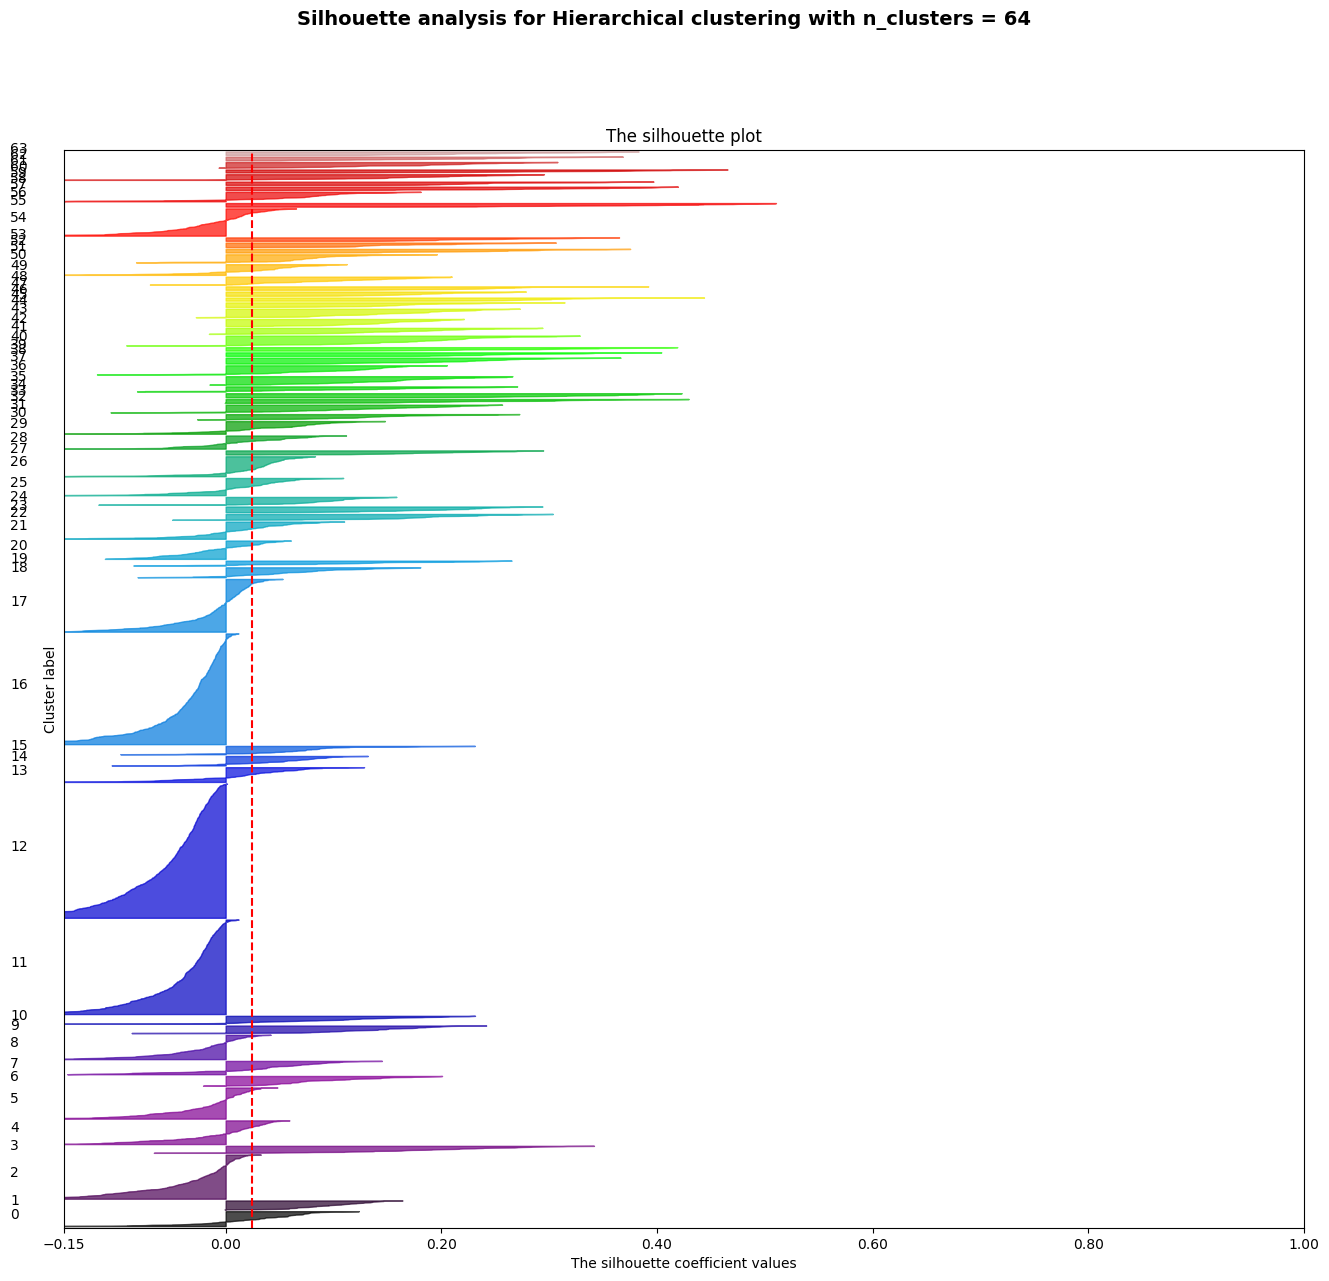
\includegraphics[width=13cm]{images/6000-64-400-Hierarchical-silhouette-plot.png}
    \caption{Silhoutte values of 6000 items clustered with 
    agglomerative clustering with Wrad's method, 64 clusters, 
    LSA with 400 components. Each pixel row corresponds to a 
    Silhouette value of an item, adjacent rows separated by gap 
    corresponds to a cluster.
    Dashed line is the average.}
    \label{fig:silh01}
  \end{center}
\end{figure}

Other measure is Calinski-Harabaz index. Clustering should be 
optimal when Calinski-Harabaz index reaches its maximum value. 
\cite{}

When evaluating the results, Silhouette Coefficient might not be
the best option. Find out why. V-measure or Adjusted Rand Index
might be better options \cite{noauthor_clustering_nodate}.


\section{``Gold standard set''}
We evaluated our clustering by creating an evaluation set with
hand labeled or verified fields of science. This subset of data 
consisted of 519 publications from three different fields. The fields
were: \emph{Computer science: Information systems}, 147 publications,
\emph{Computer science: Artificial intelligence} 153 publications, 
and \emph{Clinical neurology} 250 publications as classified by 
publisher. We checked the publisher labeling, \fixme{cleared the 
bad samples} lacking enough meta data, being too far out of the 
scope of any of the three disciplines or having corrupted data and
relabeled few \fixme{(amount)} samples to the more fitting 
discipline and to one discipline for each sample only. The ground 
truth labeling for 37 the most ambiguous samples was checked by 
a non-expert human reviewer. So, our manual classification will
be subjective but gives some hint about the classifier performance.
\fixme{Then we calculated precision and recall for the data set.} 

The Figure \ref{fig:ch-silh01} shows the results. We see that
Calinski-Harabasz index reaches it's maximum value at the number
of clusters two and that silhouette values increases with the
number of clusters.
Neither of these indices corresponds to the three disciplines
that we selected manually. It's also worth to remember that there
is only 519 data points to cluster. Comparison against preferred
manual labeling \fixme{is calculated with the 
Adjusted Rand Index (ARI) for these clusterings in Figure 
\ref{refhere}.}
Top terms for maximum index values are shown in the Table 
\ref{refhere}.

In figure \ref{fig:ch-silh02}
we see corresponding graphs for k-means clustering. Top terms for
Calinski-Harabasz index maximum at seven clusters are listed in 
the Table \ref{table:topterms}.


\begin{figure}[ht]
  \begin{center}    
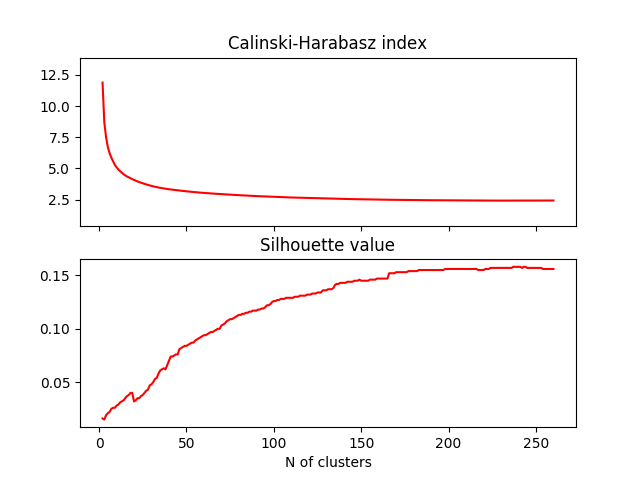
\includegraphics[width=9.5cm]{images/c-h-silh-index-plot-519-2_260-800-hierarchical.png}
    \caption{Hierarchical clustering. Calinski-Harabasz index and Silhoutte values for the
    manually annotated set of 519 publications clustered with hierarchical
    clustering, LSA with 800 components. The higher values denote 
    more compact and better clustering in both graphs.}
    \label{fig:ch-silh01}
  \end{center}
\end{figure}


\begin{figure}[ht]
  \begin{center}    
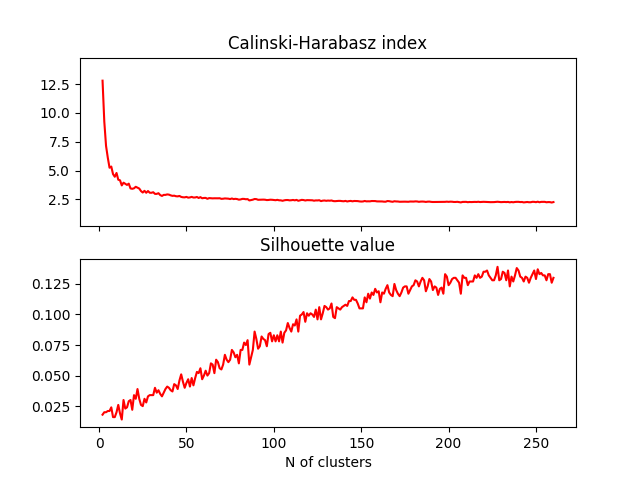
\includegraphics[width=9.5cm]{images/c-h-silh-index-plot-519-2_260-800-kmeans.png}
    \caption{k-means clustering. Calinski-Harabasz index and Silhoutte values for the
    manually annotated set of 519 publications clustered with k-means 
    clustering, LSA with 800 components. The higher values denote 
    more compact and better clustering in both graphs.}
    \label{fig:ch-silh02}
  \end{center}
\end{figure}

\begin{table}
\begin{tabular}{|p{2cm}|p{10.5cm}|} 
% Alignment of sells: l=left, c=center, r=right. 
% If you want wrapping lines, use p{width} exact cell widths.
% If you want vertical lines between columns, write | above between the letters
% Horizontal lines are generated with the \hline command:
\hline % The line on top of the table
\textbf{ } & \textbf{Top terms} \\ 
\hline 
\textbf{Cluster 0} & system internet management user project software architecture support decision business channel rule concept quality exercise  \\ 
\hline
\hline 
\textbf{Cluster 1} & lenges professional care intellectual disability people service special syndrome life child social support diagnosis pathology  \\ 
\hline
\hline 
\textbf{Cluster 2} & epilepsy stroke child seizure headache neuronal p rat sleep nerve risk treatment cell alcohol activity  \\ 
\hline
\hline 
\textbf{Cluster 3} & component filter signal neural linear bayesian ica feature value input simulation independent fuzzy vector output \\ 
\hline
\hline 
\textbf{Cluster 4} & dementia vascular ad cognitive stroke alzheimer diagnosis lesion vad risk pd brain impairment parkinson aneurysm \\ 
\hline
\hline 
\textbf{Cluster 5} & service development mobile switch agent system solution traffic environment protocol ip technology wireless game implementation \\ 
\hline
\hline 
\textbf{Cluster 6} & map image som self-organizing query logic document tree k expressive compression database retrieval rule cluster \\ 
\hline
\end{tabular} % for really simple tables, you can just use tabular
% You can place the caption either below (like here) or above the table
\caption{Top terms per cluster for manually annotated samples}
% Place the label just after the caption to make the link work
\label{table:topterms}
\end{table} % table makes a floating object with a title


\subsection{Precision and recall}
Recall is the number of items correctly classified divided by the 
total number of items in that class.
\begin{equation}
 Recall = \frac{|\{relevant\ items\} \cap \{retrieved\ items\}|} 
{\{relevant\ items\}}
\end{equation}

Precision is the number of items correctly classified divided by 
the total number items classified into that class (ie. true and 
false positives).
\begin{equation}
 Precision = \frac{|\{relevant\ items\} \cap \{retrieved\ 
items\}|} 
{\{retrieved\ items\}}
\end{equation}

With manually annotated dataset of 455 articles we compared 
the results with three clusters which was assumed the correct 
classification of the data set. We got recall $R = ???$ and 
precision $P = ???$ which is
a quite poor result. By looking at the top terms and random samples
from each cluster we notice that two of the three clusters have 
\emph{'Clinical neurology'} related items, see Tables
\ref{table:topterms_455_hier} and \ref{table:articles_455_hier}.

\begin{table}
\begin{tabular}{|p{2cm}|p{10.5cm}|} 
% Alignment of sells: l=left, c=center, r=right. 
% If you want wrapping lines, use p{width} exact cell widths.
% If you want vertical lines between columns, write | above between the letters
% Horizontal lines are generated with the \hline command:
\hline % The line on top of the table
\textbf{ } & \textbf{Top terms} \\ 
\hline 
\textbf{Cluster 1} & service image map system filter user som neural document mobile feature rule self-organizing logic query  \\ 
\hline
\hline 
\textbf{Cluster 2} & dementia vascular vad trial subcortical cognitive alzheimer criterion impairment cause lesion stroke subtypes prevalence ad  \\ 
\hline
\hline 
\textbf{Cluster 3} & stroke epilepsy pain treatment risk ad child seizure headache cognitive pd cortex parkinson cell apoe \\ 
\hline
\hline 
\end{tabular} % for really simple tables, you can just use tabular
% You can place the caption either below (like here) or above the table
\caption{Top terms for manually annotated dataset of 455 articles}
% Place the label just after the caption to make the link work
\label{table:topterms_455_hier}
\end{table} % table makes a floating object with a title

\begin{table}
\begin{tabular}{|c|p{6.5cm}|p{4.7cm}|} 
\hline % The line on top of the table
\textbf{ } & \textbf{Title} & \textbf{WoS category} \\ 
\hline 
\multirow{ 5}{*}{\textbf{1}} & Attacks against the WAP WTLS protocol & CS\_INFORMATION\_SYS \\
& Bringing knowing-when and knowing-what together: Periodically tuned categorizati & CS\_ARTIFICIAL\_INT  \\
& A digital television service architecture & CS\_INFORMATION\_SYS  \\ 
& A wavelet transform method for coding film-grain noise corrupted images & CS\_ARTIFICIAL\_INT  \\ 
& Accuracy of pedicle screw insertion with and without computer assistance: a rand & CLINICAL\_NEUROLOGY  \\
\hline
\hline 
\multirow{ 5}{*}{\textbf{2}} & Is subcortical vascular dementia a clinical entity for clinical drug trials? & CLINICAL\_NEUROLOGY \\
& Research criteria for subcortical vascular dementia in clinical trials & CLINICAL\_NEUROLOGY \\
& Subcortical vascular dementia as a specific target for clinical trials & CLINICAL\_NEUROLOGY \\ 
& Prognosis with dementia in Europe: A collaborative study of population-based coh & CLINICAL\_NEUROLOGY \\ 
& Comparison of different clinical criteria (DSM-III, ADDTC, ICD-10, NINDS-AIREN, & CLINICAL\_NEUROLOGY \\
\hline
\hline 
\multirow{ 5}{*}{\textbf{3}} & Interferon-alpha 2a effects on complement activation and regulation in MS patien & CLINICAL\_NEUROLOGY \\
& Architectural evolution - Nokia mobile phone case & CS\_INFORMATION\_SYS \\
& CASCADE: A European collaborative study on vascular determinants of brain lesion & PUBL\_ENVTL\_OCCUPA  \\ 
& Natural history of unruptured intracranial aneurysms: probability of and risk fa & CLINICAL\_NEUROLOGY \\ 
& An FDOPA PET study in patients with periodic limb movement disorder and restless & CLINICAL\_NEUROLOGY \\
\hline
\hline 
\end{tabular} % for really simple tables, you can just use tabular
\caption{Five random articles per cluster for manually annotated dataset of 455 articles}
\label{table:articles_455_hier}
\end{table} % table makes a floating object with a title



\subsection{Other metrics}
Different metrics to evaluate clustering include (from 
scikit-learn) Adjusted Rand Index, Mutual Information scores 
(NMI, AMI), homogenity, completness, V-measure, Fowlkes-Mallows 
scores, Silhouette Coefficient, Calinski-Harabaz Index, (from 
sources) 


\section{Finnish publications from year 2000}
We clustered year 2000 data, 10145 publications, with k-means 
clustering with different value of $k$, the number of clusters. 
The Figure \ref{fig:ch-silh02} shows the results.
\begin{figure}[ht]
  \begin{center}    
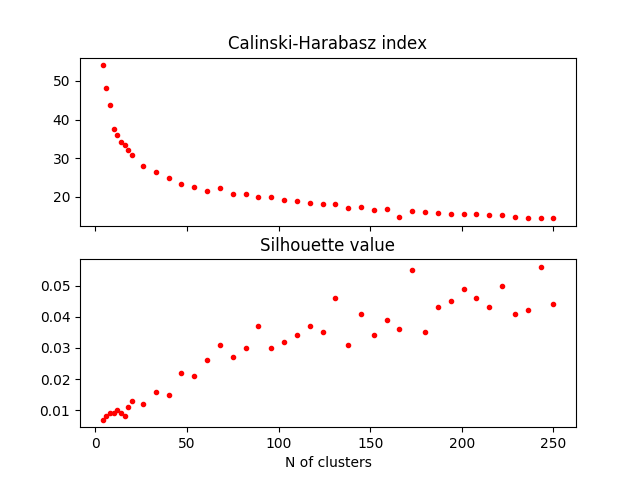
\includegraphics[width=10cm]{images/c-h-silh-index-plot-y2000-2_260-800-kmeans.png}
    \caption{Calinski-Harabasz index and Silhoutte values of 
10145 items clustered with k-means clustering, LSA with 800 
components. The higher values denote more compact and better 
clustering in both graphs.}
    \label{fig:ch-silh02}
  \end{center}
\end{figure}

Similarly the same data was clustered with agglomerative 
hierarchical Ward's clustering by sampling the number of clusters 
from the values [2-260]. The silhouette and Calinski-Harabasz values
are shown in Figure \ref{}
\begin{figure}[ht]
  \begin{center}    
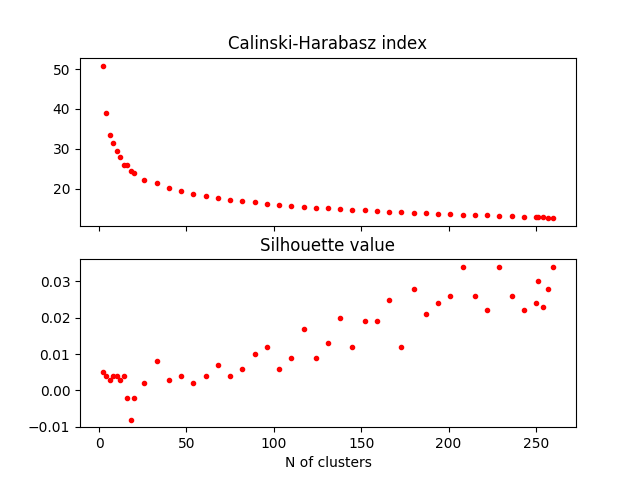
\includegraphics[width=10cm]{images/c-h-silh-index-plot-y2000-2_260-800-hierarchical.png}
    \caption{Hierarchical clustering. Calinski-Harabasz index and Silhoutte values for the
    Finnish publications from year 2000 clustered with hierarchical
    clustering, LSA with 800 components. The higher values denote 
    more compact and better clustering in both graphs.}
    \label{fig:ch-silh-2000-01}
  \end{center}
\end{figure}
We can see from the values that they prefer different features in
the data. Calinski-Harabasz index sees the fewest number of 
clusters - two - as the most compact and optimal clustering. Also
the form of the curve hints to perhaps power law that is also 
known as Zipf's law in text analysis. \fixme{Check this.}
It should be noticed that the silhouette values are quite low 
in absolute terms considering it's index space [-1,1]. This might 
be in line with the fact that it's best suited for [normally?] 
distributed and compact clusters. But we can also see that the 
silhouette values grow with the number of clusters although no
maxima seems to be reached with these cluster values.











 
\chapter{Discussion}
\label{chapter:discussion}

The usefulness of our results lies in that they show how difficult
the task at hand is, and what aspects there are to consider when
approaching the problem.
% Alkuasetelma
The problem of defining how the science should be classified into
different disciplines is quite difficult and ambiguous.

% Datasta
The data was incomplete but we chose to use it as such without 
pruning the possible defective samples. This was due to the 
amount of data, manually checking over 20000 titles was not an 
option and sufficient general rules to filter the data did not 
occur to us in the beginning of the work. Some minimum length for 
the publication data could leave out clearly inadequate samples 
and perhaps improve the clustering results. General outlier 
detection techniques \cite{hodge_survey_2004} could prove 
problematic here when there obviously will be single publications 
in some disciplines. There probably would be disciplines with very
few publications in spite of including more data.

% Datan määrästä
We tried to include a larger data set, covering years 2000-2003, 
$47303$ publications, to cluster. This resulted running out of 
memory in our laptop environment with 16 GB of RAM. Obviously more 
capacity would have been available but taking over a new 
environment was not possible within the limits of this work.

% Piirreirroituksesta
Tokenization during pre-processing left one and two character 
words such as measurement units in data which was not desired. 
Adjusting tokenization or extending the stop word list should 
filter these out. 
During vectorisation we hit our limit of maximum number of terms 
of $50000$. This might be undesirable because now our terms were
from the most frequent end of the frequency range of minimum $2$ 
occurrences -- maximum in $10\ \%$ of documents. This means that 
rarer and thus more specific terms might have been discarded.
We tested some hand picked values of minimum and maximum document 
frequency threshold for terms but more systematic exploration of 
these parameters could give better set of features.
%- \fixme{``Suositus...'' ``Nämä parametriarvot...''}
Furthermore, the discarded terms contained quite many compounds 
joined with underscore '\_' to conserve the constructs. It might 
be worth to try and split those compounds to enable the individual 
words to be counted. On the other hand, using 2-grams or higher 
order n-grams in addition to single words could also be 
interesting to try, although it will again increase the number terms.

% Ulottuvuuksien vähentämisestä
Selected number of components in reducing dimensionality of the 
data resulted quite low proportion of explained variance (35 \%).
%seemed to retain enough information while also allowing to run clusterings fast enough.
On the other hand, the resulting $800$ component low-dimensional
space is quite high dimensional too.
With the manually annotated data set the explained variance was 
$100\ \%$. Yet the internal validation metrics gave insignificant 
values. This probably shows that $800$ dimensional data with just 
$455$ samples is still too high dimensional \cite{aggarwal_surprising_2001}. 
Selecting and extracting features more carefully and then reducing
dimensionality more could help. Transforming data somewhere to 
$[50-150]$ components could be more justified range 
\cite{dolnicar_review_2002}. Overall using more data such as whole
world data could improve clustering results.

% Model selection
The model selected, agglomerative Ward's clustering, is one of the
basic clustering methods. We selected it because it produces 
hierarchical cluster structure that is naturally expected of fields
and sub fields of science. The method should also tolerate noise 
somewhat.
% while failing ...
It is known to work well only with compact, even-sized clusters.
This might be a problem with the current data where different 
disciplines are expected to be varying in size.
It can't cluster very large data sets because of the computational
cost. We might have bumped to that limit in a smaller scale while 
trying to cluster the four year data of ~47000 publications.
The selected model is a hard clustering method in a sense that a
publication is clustered to one discipline explicitly.


% Choosing the number of clusters
Choosing the number of clusters was a difficult part of this 
problem. We tried two internal validation methods,
Calinski-Harabasz criterion and silhouette values. Neither of them
could reveal any meaningful optimal clustering if any occurred.
Our manually annotated data set for choosing the number of clusters
was probably too small ($455$) compared to number of components 
($800$). 
It has been also noted that Calinski-Harabasz index 
might suffer even from moderate noise \cite{liu_understanding_2010}.
There are other internal clustering validation metrics that might 
work better with our data, one perhaps worth testing could be
S\_Dbw (Scatter and Density between clusters) index 
\cite{halkidi_clustering_2001}. 
It might also be that the merging of two computer science related 
sub fields into one cluster and clinical neurology splitting into 
two clusters can also result from the true properties of the data.
Perceived human definitions might not always match up with the 
underlying data. So there might be two sectors of clinical 
neurology represented in the data that are more distant from each 
other than these publications related to two computer science fields.

% Itse klusteroinnista
We didn't utilize the hierarchical structure of agglomerative 
clustering in this work. 
% We tried but didn't have time and didn't manage to to find out 
% how to extract and use the structure data.
It could have helped in deciding the number of clusters \cite{kimes_statistical_2017}.
% - Compared to current classification of articles into fields of 
% science based on WoS classification...

% Vertailu aiempaa suomalaiseen vastaavaan ``Suominen... et al.''
We could have very roughly compared our clustering to existing 
classification by calculating adjusted Rand index against WoS 
subject categories.
The question there would be how to automatically select WoS 
category for comparison for a publication that has several 
categories.

\section*{Conclusions}
\label{sec:conclusions}
We tried a basic agglomerative clustering with Ward's method on 
Finnish publications from years 2000-2001 to see if meaningful 
clustering by scientific discipline could be obtained. Some 
sensible clusters might have been formed but there appeared also 
totally mixed clusters which reduces the overall result as 
unsatisfactory.
% Toteutuksen heikkoudet ja vahvuudet
The clustering method was tested to the limit of our laptop 
environment with the amount of data.

Future work should improve the pre-processing of the data, consider 
using larger data set and test hybrid models mixing both text and
citation analysis. Relaxing the hard clustering assumption to 
allow for soft clustering of probability based discipline labelling
could also prove interesting.

 
\chapter{Conclusions}
\label{chapter:conclusions}

Two to four pages might be a good limit. 



% Load the bibliographic references
% ------------------------------------------------------------------
% You can use several .bib files:
% \bibliography{sources,ietf_sources}
\bibliography{v_lahteet,dippa_luettavat,victor11}


% Appendices go here
% ------------------------------------------------------------------
% If you do not have appendices, comment out the following lines
%\appendix
%\chapter{Manually annotated data set}
\label{chapter:first-appendix}

Title, resulting classification and taken decision of manually 
annotated publications.

\pgfplotstabletypeset[
    col sep=semicolon,
    verb string type,
    begin table=\begin{longtable},
    end table=\end{longtable},
    columns={Title, My class name, Clarification 3},
    columns/Title/.style={column name=Title, column type={|p{60mm}}},
    columns/My class name/.style={column name=Discipline, column type={|p{36mm}}},
    columns/Clarification 3/.style={column name=Clarification, column type={|p{28mm}|}},
    every even row/.style={before row={\rowcolor[gray]{0.9}}},
    every head row/.style={before row=\hline,after row=\hline},
    every head row/.append style={after row=\endhead},    
    every last row/.style={after row=\hline},
    ]{../data/baseline/groundtruth_labels_CS-AI-IS_CN_for_appendix.csv}

 
\chapter{Top terms}
\label{chapter:second-appendix}

\pgfplotstabletypeset[
    col sep=colon,
    verb string type,
    begin table=\begin{longtable},
    end table=\end{longtable},
%     label=\label{table:topterms\_hier}
    columns/cluster/.style={column name={Cluster}, column type={|l}},
    columns/top terms/.style={column name={Top terms}, column type={|p{115mm}|}},
    every even row/.style={before row={\rowcolor[gray]{0.9}}},
    every head row/.style={before row=\hline,after row=\hline},
    every head row/.append style={after row=\endhead},
    every last row/.style={after row=\hline}
]{../data/processed/topterms/12000-188-800-hierarchical-topterms.csv}



% End of document!
% ------------------------------------------------------------------
% The LastPage package automatically places a label on the last page.
% That works better than placing a label here manually, because the
% label might not go to the actual last page, if LaTeX needs to place
% floats (that is, figures, tables, and such) to the end of the 
% document.
\end{document}
